\section{Pyramid Supplement}
\label{app:pyrappendix}

\begin{figure}[!ht]
\begin{center}
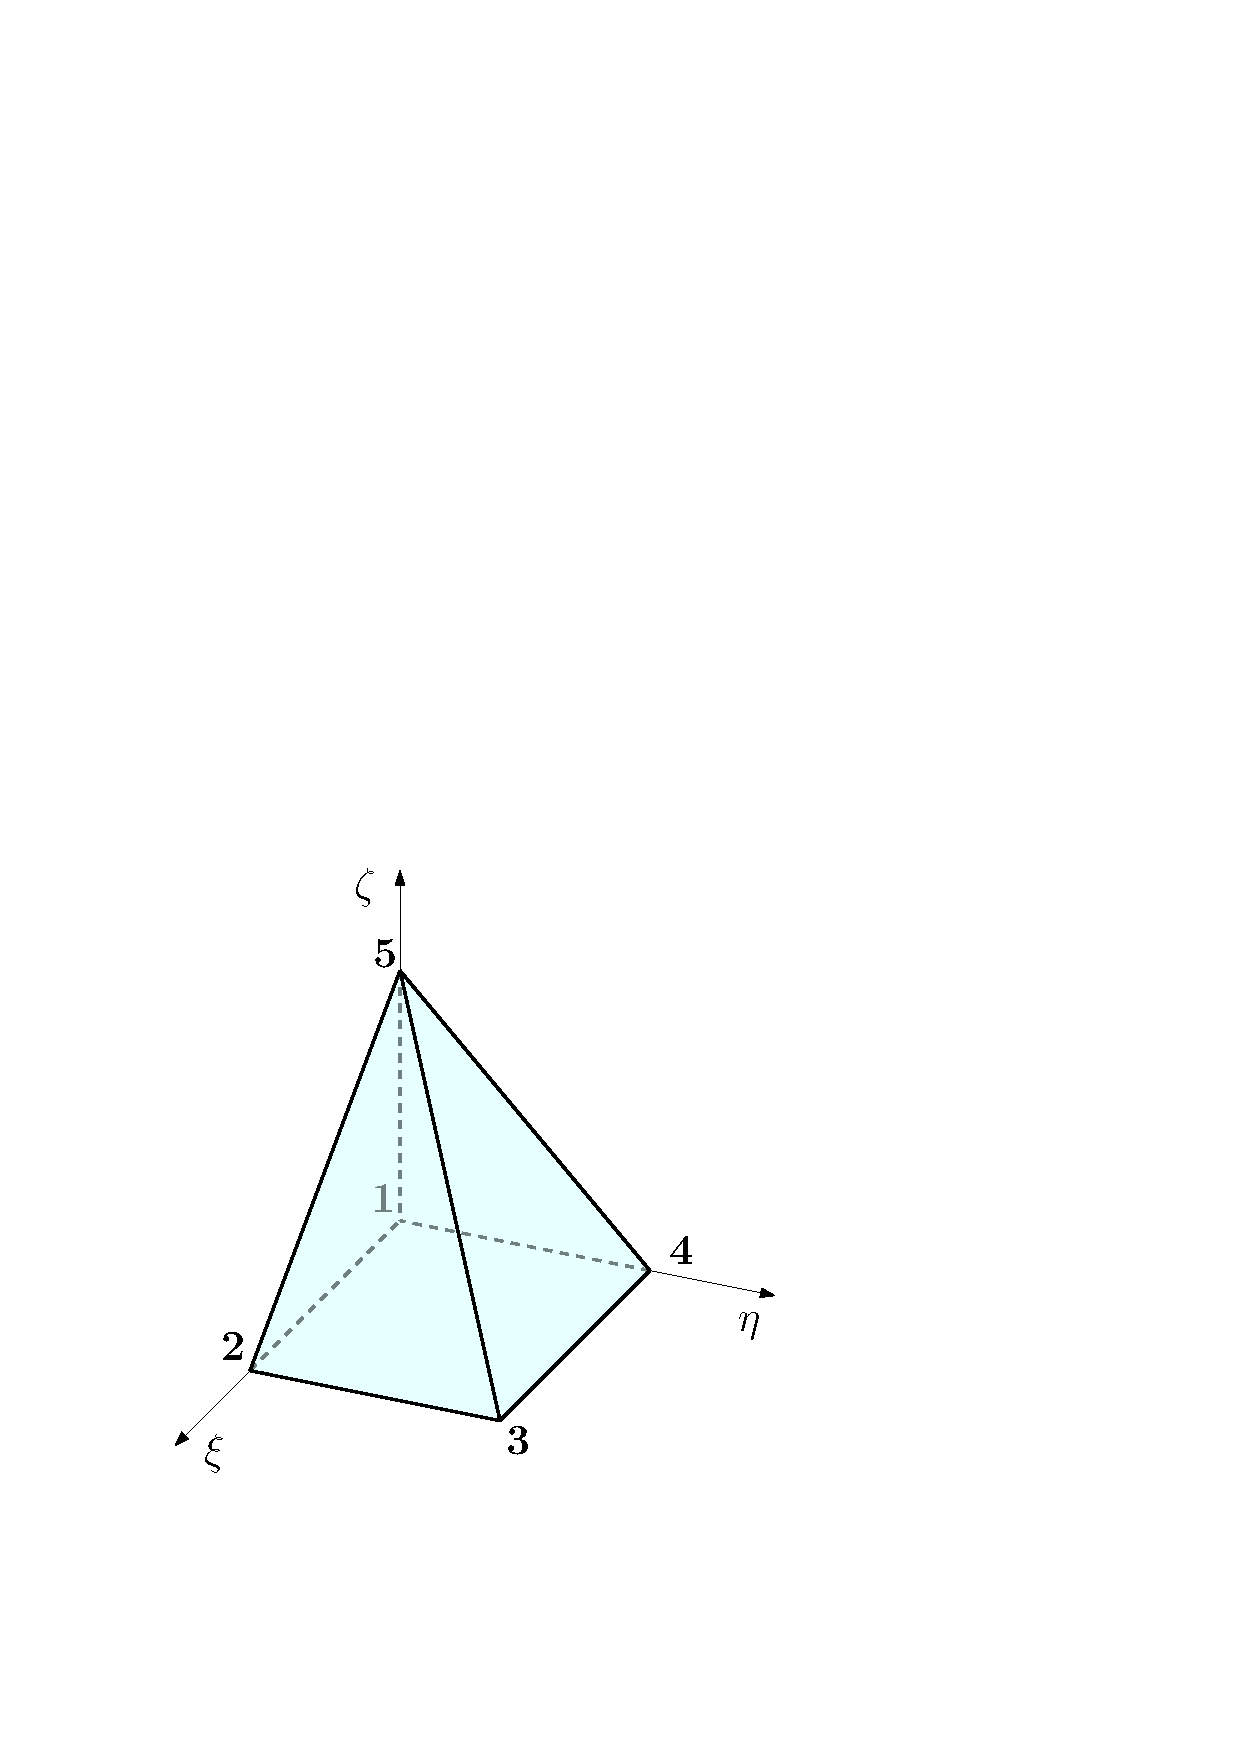
\includegraphics[scale=0.5]{./figures/MasterPyramidAppendix.pdf}
\caption{Master pyramid with numbered vertices.}
\label{fig:MasterPyramidAppendix}
\end{center}
\end{figure}

The master pyramid is shown in Figure \ref{fig:MasterPyramidAppendix} in the $(\xi,\eta,\zeta)$ space (\textit{not} the $(\xi_1,\xi_2,\zeta)$ space).
More specifically, the definition is $\Omega=\{(\xi,\eta,\zeta)\in\R^3:\xi>0,\eta>0,\zeta>0,\xi+\zeta<1,\eta+\zeta<1\}$.

This supplement provides the proofs that the pyramid shape functions proposed in \S\ref{sec:Pyramid} are in the finite element spaces  defined in the fundamental work by \citet{Nigam_Phillips_11}.
%These discrete spaces are defined in the fundamental work by \citet{Nigam_Phillips_11}.
Recall from \eqref{eq:pyramidsequence} that the discrete spaces forming the exact sequence are $\mathcal{U}^{(m),p}$ for $m=0,1,2,3$, where $m$ stands for the differential $m$-forms lying in each space.
The spaces $\mathcal{U}^{(m),p}$ are defined as
\begin{equation}
	\mathcal{U}^{(m),p}=\mathcal{V}^{(m),p}\cap\Gamma^{(m),p}\,,
\end{equation}
where the spaces $\mathcal{V}^{(m),p}$ are called the \textit{underlying spaces}, and the spaces $\Gamma^{(m),p}$ are called the \textit{compatibility spaces}.
These two families of spaces will be defined next.

First, note that the compatibility spaces ensure the elements in $\mathcal{U}^{(m),p}$ are compatible at the level of spaces with the other elements.
Indeed, they consist of those functions having their face traces lying on the appropriate 2D quadrilateral and triangle spaces in \eqref{eq:QuadES} and \eqref{eq:EStriangle} respectively.
More specifically, let $\mathrm{tr}_\Tri^{(m)}$ and $\mathrm{tr}_\square^{(m)}$ be the trace of the differential $m$-forms over the four pyramid triangle faces and the pyramid quadrilateral face respectively.
Recall that for $m=0$ the trace is the value of the function itself, for $m=1$ the trace is the 2D tangential component, while for $m=2$ the trace is the normal component.
With this in mind, the compatibility spaces are,\footnote{Note that in \eqref{eq:Pyramidcompatilibityspaces}, the very special property that $\mathcal{P}^p$, $\mathcal{N}^p$ and $\mathcal{RT}^p$ are affine invariant is used. If the spaces were different, one would need to take the 2D pullback of each triangle trace to the master triangle. The same holds for the quadrilateral trace, where in this case it is exploited that the quadrilateral face is the master quadrilateral and no transformation is needed.}
\begin{equation}
\begin{aligned}
	\Gamma^{(0),p}&=\{\phi\in H^1:\mathrm{tr}_\Tri^{(0)}(\phi)\in\mathrm{tr}_\Tri^{(0)}(\mathcal{P}^p(\xi,\eta,\zeta)),\,\,
		\mathrm{tr}_\square^{(0)}(\phi)\in\mathcal{Q}^{p,p}(\xi,\eta)\}\,,\\
%			\mathrm{tr}_\square^{(0)}(\mathcal{Q}^{p,p,p})\}\,,\\
	\Gamma^{(1),p}&=\{E\in H(\mathrm{curl}):\mathrm{tr}_\Tri^{(1)}(E)\in\mathrm{tr}_\Tri^{(1)}(\mathcal{N}^p(\xi,\eta,\zeta)),\,\,
		\mathrm{tr}_\square^{(1)}(E)\in\mathcal{Q}^{p-1,p}(\xi,\eta)\!\times\!\mathcal{Q}^{p,p-1}(\xi,\eta)\}\,,\\
%			\mathrm{tr}_\square^{(1)}(\mathcal{Q}^{p-1,p,p}\times\mathcal{Q}^{p,p-1,p}\times\mathcal{Q}^{p,p,p-1})\}\,,\\
	\Gamma^{(2),p}&=\{V\in H(\mathrm{div}):\mathrm{tr}_\Tri^{(2)}(V)\in\mathrm{tr}_\Tri^{(2)}(\mathcal{RT}^p(\xi,\eta,\zeta)),\,\,
		\mathrm{tr}_\square^{(2)}(V)\in\mathcal{Q}^{p-1,p-1}(\xi,\eta)\}\,,\\
%			\mathrm{tr}_\square^{(2)}(\mathcal{Q}^{p,p-1,p-1}\times\mathcal{Q}^{p-1,p,p-1}\times\mathcal{Q}^{p-1,p-1,p})\}\,,\\
	\Gamma^{(3),p}&=\{\psi\in L^2\}\,.
\end{aligned}
\label{eq:Pyramidcompatilibityspaces}
\end{equation}
%Note that $\mathcal{Q}^{p,p}(\xi,\eta)=\mathrm{tr}_\square^{(0)}(\mathcal{Q}^{p,p,p}(\xi,\eta,\zeta))$ and similarly with $m=1,2$.

Fortunately, at the level of shape functions, dealing with the compatibility spaces is not as intimidating as it might look.
All that is required is that the shape functions satisfy the dimensional hierarchy, so that their nonzero face traces correspond to the lower dimensional shape functions, which are known to lie in the correct space.
Therefore, if a shape function satisfies the required trace properties, it \textit{automatically} belongs to the appropriate compatibility space.

The main difficulty lies in showing that the shape functions belong to the underlying spaces $\mathcal{V}^{(m),p}$.
In fact, these spaces are not nicely defined directly on the master pyramid.
For this reason, it is more convenient to define them on a deformed space where the symmetries are more evident, and then use the inverse pullback to the master pyramid.
This process is explained in what follows.

%Instead of defining them directly on the master pyramid, the spaces are defined on a deformed space where the symmetries are more evident, and then mapped back to the master pyramid.
%This is a typical approach.
%The deformed space is usually chosen as a cube, but \citet{Nigam_Phillips_11} chose it to be an \textit{infinite pyramid}, which is defined as $\Omega_\infty=\{(x,y,z)\in\R^3:0<x<1,0<y<1,z>0\}$.
%The necessary concepts to define the spaces are presented in what follows.
%%before presenting the definition, some preliminary concepts are required first.
%%These discrete spaces are not defined yet, and defining them will be the next mission.

\begin{figure}[!ht]
\begin{center}
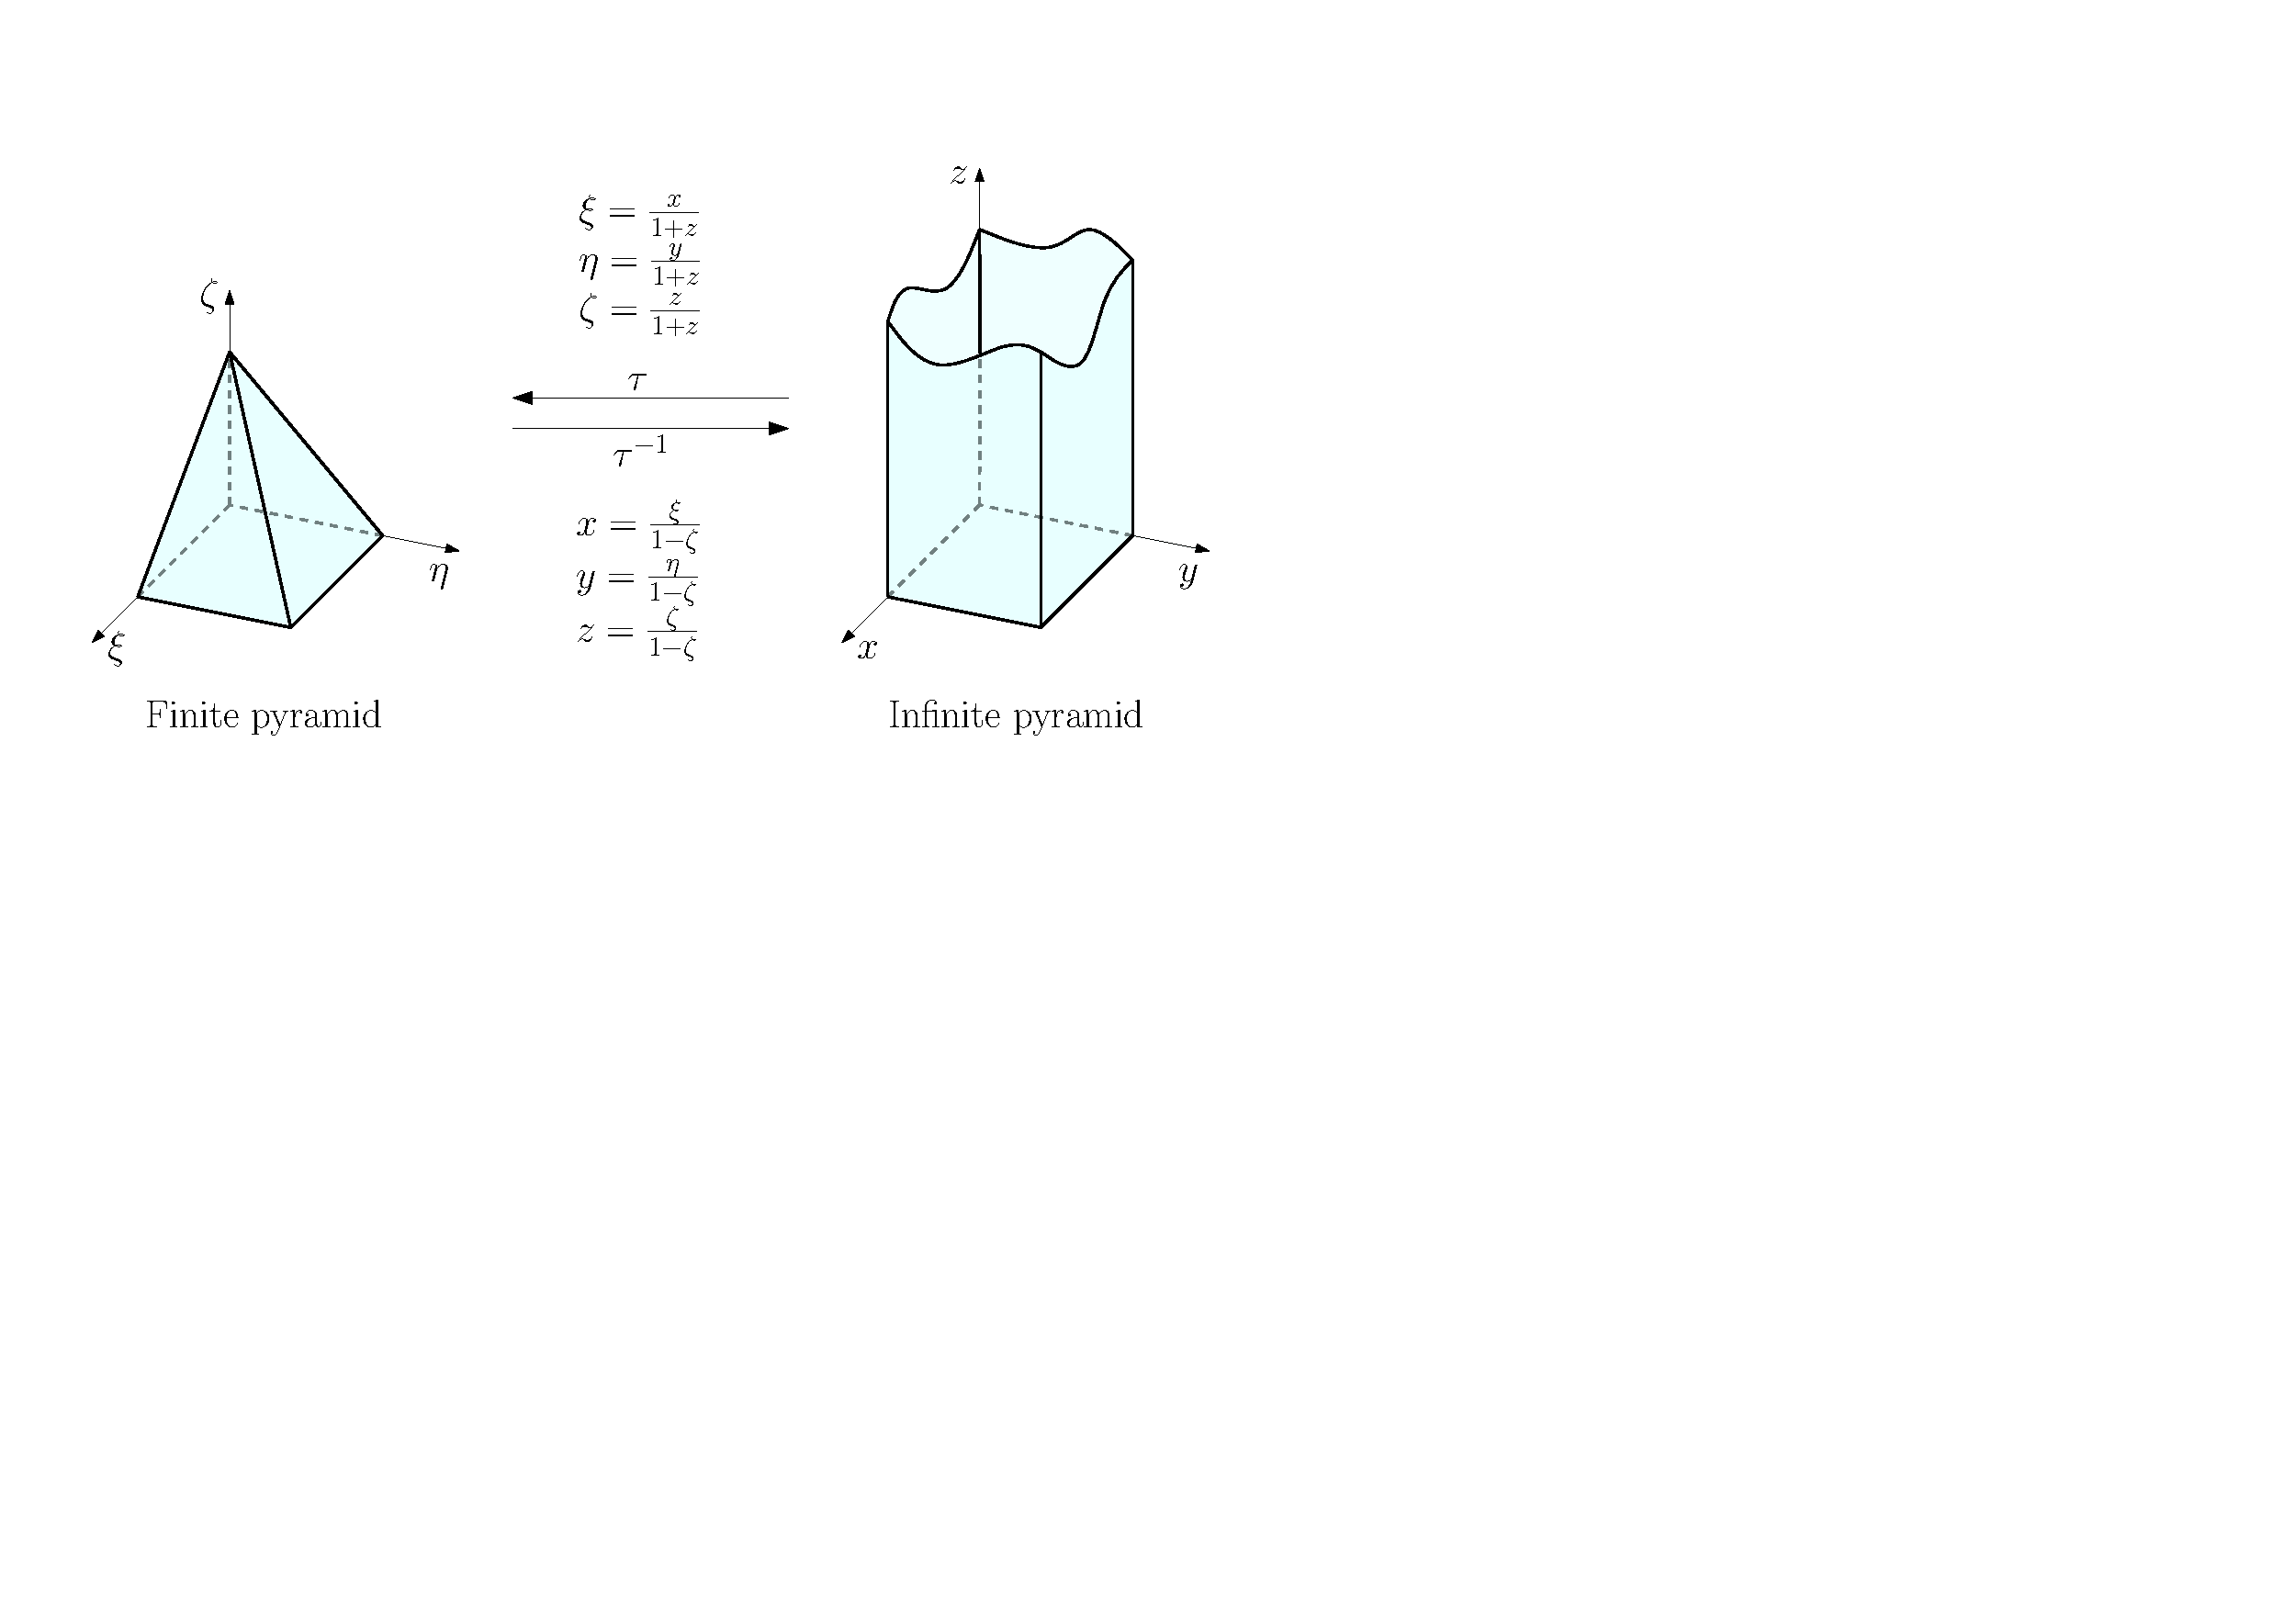
\includegraphics[scale=0.5]{./figures/PyramidSingleTransform.pdf}
\caption{Transformation from the infinite pyramid to the master pyramid.}
\label{fig:PyramidSingleTransform}
\end{center}
\end{figure}

The deformed space is usually chosen as a cube, but \citet{Nigam_Phillips_11} chose it to be an \textit{infinite pyramid}, which is defined as $\Omega_\infty=\{(x,y,z)\in\R^3:0<x<1,0<y<1,z>0\}$.
The first step is to consider the transformation $\tau:\Omega_\infty\rightarrow\Omega$ from the intinite pyramid $\Omega_\infty$ to the pyramid $\Omega$, which is given by the component equations,
\begin{equation}
	\xi=\frac{x}{1+z},\quad\qquad\eta=\frac{y}{1+z},\quad\qquad\zeta=\frac{z}{1+z}\,.
\end{equation}
Clearly, $\tau$ is a diffeomorphism between these open sets (\textit{not} when including the boundary).
The inverse $\tau^{-1}:\Omega\rightarrow\Omega_\infty$ is given by the component equations,
\begin{equation}
	x=\frac{\xi}{1-\zeta},\quad\qquad y=\frac{\eta}{1-\zeta},\quad\qquad z=\frac{\zeta}{1-\zeta}\,.
\end{equation}
The transformation is depicted in Figure \ref{fig:PyramidSingleTransform}.
Take note of the following useful expressions resulting from this transformation,
\begin{equation*}
	1-x=\frac{1-\xi-\zeta}{1-\zeta},\quad\quad 1-y=\frac{1-\eta-\zeta}{1-\zeta},\quad\quad
	1+z=\frac{1}{1-\zeta},\quad\quad \frac{1}{1+z}=1-\zeta\,.
\end{equation*}

Next consider the following isomorphic mappings,
\begin{equation}
\begin{aligned}
	\tau^{-*,(m)}:&\mathcal{V}_\infty^{(m),p}\longrightarrow\mathcal{V}^{(m),p}=\tau^{-*,(m)}(\mathcal{V}_\infty^{(m),p})\,,\\
		\tau^{*,(m)}:&\mathcal{V}^{(m),p}\longrightarrow\mathcal{V}_\infty^{(m),p}\,,
\end{aligned}
\end{equation}
where $\tau^{-*,(m)}$ and $\tau^{*,(m)}$ are the inverse pullback and pullback mappings induced by $\tau$.
Since the spaces $\mathcal{V}^{(m),p}$ and $\mathcal{V}_\infty^{(m),p}$ are isomorphic, it is mathematically irrelevant which of the two spaces is actually defined, since the other space can be determined through the corresponfing pullback mapping.
However, sometimes there are practical reasons to explicitly define one set of spaces over the other.
Indeed, it is more opportune to define the deformed underlying spaces $\mathcal{V}_\infty^{(m),p}$, which are\footnote{Note there is misprint in \citet{Nigam_Phillips_11} in (3.8) when presenting the equivalent characterization of $\mathcal{V}_\infty^{(1),p}$. The definition here corrects that, and is consistent with the calculations in \S3.3 of \citet{Nigam_Phillips_11}.}
\begin{equation}
\begin{aligned}
	\mathcal{V}_\infty^{(0),p}&=\{\phi\!\in\!\mathcal{Q}_p^{p,p,p}:
		\nabla\phi\!\in\!\mathcal{Q}_p^{p-1,p,p-1}\!\times\!\mathcal{Q}_p^{p,p-1,p-1}\!\times\!\mathcal{Q}_{p+1}^{p,p,p-1}\}\,,\\
	\mathcal{V}_\infty^{(1),p}&=\{E\!\in\!
		\mathcal{Q}_{p+1}^{p-1,p,p}\!\times\!\mathcal{Q}_{p+1}^{p,p-1,p}\!\times\!\mathcal{Q}_{p+1}^{p,p,p-1}:
			\nabla\!\times\! E\!\in\!
				\mathcal{Q}_{p+2}^{p,p-1,p-1}\!\times\!\mathcal{Q}_{p+2}^{p-1,p,p-1}\!\times\!\mathcal{Q}_{p+1}^{p-1,p-1,p-1}\}\,,\\
	\mathcal{V}_\infty^{(2),p}&=\{V\!\in\!
		\mathcal{Q}_{p+2}^{p,p-1,p-1}\!\times\!\mathcal{Q}_{p+2}^{p-1,p,p-1}\!\times\!\mathcal{Q}_{p+2}^{p-1,p-1,p}:
			\nabla\cdot V\!\in\!\mathcal{Q}_{p+3}^{p-1,p-1,p-1}\}\,,\\
	\mathcal{V}_\infty^{(3),p}&=\{\psi\!\in\!\mathcal{Q}_{p+3}^{p-1,p-1,p-1}\}\,,
\end{aligned}
\end{equation}
where $\mathcal{Q}_{n}^{p,q,r}=\mathcal{Q}_{n}^{p,q,r}(x,y,z)$ are the $n$-weighted tensor polynomial spaces. 
They are defined as
\begin{equation}
	\mathcal{Q}_{n}^{p,q,r}(x,y,z)
		=\Big\{\frac{\psi(x,y,z)}{(1+z)^n}:\psi(x,y,z)\in\mathcal{Q}^{p,q,r}(x,y,z)\Big\}\,.
\end{equation}
Note the useful inclusion $\mathcal{Q}_{n}^{p,q,r}\subseteq\mathcal{Q}_{n+1}^{p,q,r+1}$ which holds for these rational polynomial spaces.

Lastly, note that the pullbacks $\tau^{*,(m)}$ take different forms depending on $m$.
Indeed, if $J_\tau$ is the Jacobian of the transformation $\tau$, the pullbacks are,
\begin{equation}
\begin{alignedat}{3}
	\tau^{*,(0)}\phi&=\phi\circ\tau\,,\quad&&\phi\in H^1\,,\\
	\tau^{*,(1)}E&=J_\tau^{\T}(E\circ\tau)\,,\quad && E\in H(\mathrm{curl})\,,\\
	\tau^{*,(2)}V&=\det(J_\tau)J_\tau^{-1}(V\circ\tau)\,,\quad && V\in H(\mathrm{div})\,,\\
	\tau^{*,(3)}\psi&=\det(J_\tau)(\psi\circ\tau)\,,\quad && \psi\in L^2\,.
\end{alignedat}
\label{eq:pullbacksgeneral}
\end{equation}
The same relations hold for the inverse pullbacks $\tau^{-*,(m)}$, but replacing $\tau$ by $\tau^{-1}$, $J_\tau$ by $J_{\tau^{-1}}$, and the domains by their isometrically isomorphic counterparts,\footnote{The spaces are iso\textit{metrically} isomorphic if the appropriate weights are added to the definition of the norm.} $H_\infty^1=\tau^{*,(0)}(H^1)$, $H(\mathrm{curl})_\infty=\tau^{*,(1)}(H(\mathrm{curl}))$, $H(\mathrm{div})_\infty=\tau^{*,(2)}(H(\mathrm{div}))$, and $L_\infty^2=\tau^{*,(3)}(L^2)$.
Even though they will be unnecessary, in the interest of completeness these pullback mappings are written explicitly below,
\begin{equation}
\begin{alignedat}{3}
	\tau^{*,(0)}\phi&=\phi\circ\tau\,,\quad
		&&\phi\in H^1\,,\\
	\tau^{*,(1)}E&=\frac{1}{(1+z)^2}\begin{pmatrix}1+z&0&0\\0&1+z&0\\-x&-y&1\end{pmatrix}(E\circ\tau)\,,\quad
		&& E\in H(\mathrm{curl})\,,\\
	\tau^{*,(2)}V&=\frac{1}{(1+z)^3}\begin{pmatrix}1&0&x\\0&1&y\\0&0&1+z\end{pmatrix}(V\circ\tau)\,,\quad
		&& V\in H(\mathrm{div})\,,\\
	\tau^{*,(3)}\psi&=\frac{1}{(1+z)^4}(\psi\circ\tau)\,,\quad
		&&\psi\in L^2\,.
\end{alignedat}
\label{eq:Pyramidpullbacks}
\end{equation}
The inverse pullbacks explicitly are,
\begin{equation}
\begin{alignedat}{3}
	\tau^{-*,(0)}\phi&=\phi\circ\tau^{-1}\,,\quad 
		&&\phi\in H_\infty^1\,,\\
	\tau^{-*,(1)}E&=\frac{1}{(1-\zeta)^2}\begin{pmatrix}1-\zeta&0&0\\0&1-\zeta&0\\\xi&\eta&1\end{pmatrix}(E\circ\tau^{-1})\,,\quad 
		&& E\in H(\mathrm{curl})_\infty\,,\\
	\tau^{-*,(2)}V&=\frac{1}{(1-\zeta)^3}\begin{pmatrix}1&0&-\xi\\0&1&-\eta\\0&0&1-\zeta\end{pmatrix}(V\circ\tau^{-1})\,,\quad 
		&& V\in H(\mathrm{div})_\infty\,,\\
	\tau^{-*,(3)}\psi&=\frac{1}{(1-\zeta)^4}(\psi\circ\tau^{-1})\,,\quad 
		&&\psi\in L_\infty^2\,.
\end{alignedat}
\label{eq:Pyramidinversepullbacks}
\end{equation}

To prove the shape functions defined in \S\ref{sec:Pyramid} are in the underlying spaces, in general one would pull them back (using \eqref{eq:Pyramidpullbacks}) and check if they belong to the spaces $\mathcal{V}_\infty^{(m),p}$.
However, due to the \textit{coordinate free} definitions of the ancillary functions and the shape functions in general, it is not necessary to find the pullback explicitly.
Instead, one simply finds the trivial pullback of all the sets of affine coordinates and their gradients in the $(x,y,z)$ coordinates.
Then, the only task is to evaluate all the shape functions with these affine coordinates and the result will be the desired pullback of the original shape function.
This is why the mappings \eqref{eq:Pyramidpullbacks} and \eqref{eq:Pyramidinversepullbacks} become redundant for our shape functions.

In view of these comments, it is useful to have all the affine coordinates and their gradients in the $(x,y,z)$ space.
The triangle affine coordinates (see \eqref{eq:PyramidTriCoord}) are
\begin{equation}
	\begin{gathered}
		\nu_0(x,z)=\sxxz\,,\qquad\nu_1(x,z)=\sxz\,,\qquad\nu_2(z)=\szzz\,,\\
		\nu_0(y,z)=\syyz\,,\qquad\nu_1(y,z)=\syz\,,\qquad\nu_2(z)=\szzz\,.
	\end{gathered}
\end{equation}
Their gradient (see \eqref{eq:PyramidTriCoordGrad}) is
\begin{equation}
	\begin{gathered}
		\nabla\nu_0(x,z)=\textstyle{\frac{1}{(1+z)^2}}\bigg(\begin{smallmatrix}-(1+z)\\[2pt]0\\[2pt]-(1-x)\end{smallmatrix}\bigg)\,,\qquad
			\nabla\nu_1(x,z)=\textstyle{\frac{1}{(1+z)^2}}\bigg(\begin{smallmatrix}(1+z)\\[2pt]0\\[2pt]-x\end{smallmatrix}\bigg)\,,\qquad
				\nabla\nu_2(z)=\textstyle{\frac{1}{(1+z)^2}}\bigg(\begin{smallmatrix}0\\[2pt]0\\[2pt]1\end{smallmatrix}\bigg)\,,\\
		\nabla\nu_0(y,z)=\textstyle{\frac{1}{(1+z)^2}}\bigg(\begin{smallmatrix}0\\[2pt]-(1+z)\\[2pt]-(1-y)\end{smallmatrix}\bigg)\,,\qquad
			\nabla\nu_1(y,z)=\textstyle{\frac{1}{(1+z)^2}}\bigg(\begin{smallmatrix}0\\[2pt](1+z)\\[2pt]-y\end{smallmatrix}\bigg)\,,\qquad
				\nabla\nu_2(z)=\textstyle{\frac{1}{(1+z)^2}}\bigg(\begin{smallmatrix}0\\[2pt]0\\[2pt]1\end{smallmatrix}\bigg)\,.
	\end{gathered}
\end{equation}
The sets of quadrilateral scaled 1D affine coordinates (see \eqref{eq:PyramidQuadCoord}) are
\begin{equation}
	\begin{gathered}
		\mu_0(x)=1-x\,,\quad\qquad\mu_1(x)=x\,,\\
		\mu_0(y)=1-y\,,\quad\qquad\mu_1(y)=y\,.
	\end{gathered}
\end{equation}
Their gradient (see \eqref{eq:PyramidQuadCoordGrad}) is
\begin{equation}
	\begin{gathered}
		\nabla\mu_0(x)=\bigg(\begin{smallmatrix}-1\\[2pt]0\\[2pt]0\end{smallmatrix}\bigg)\,,\quad\qquad
    	\nabla\mu_1(x)=\bigg(\begin{smallmatrix}1\\[2pt]0\\[2pt]0\end{smallmatrix}\bigg)\,,\\
		\nabla\mu_0(y)=\bigg(\begin{smallmatrix}0\\[2pt]-1\\[2pt]0\end{smallmatrix}\bigg)\,,\quad\qquad
    	\nabla\mu_1(y)=\bigg(\begin{smallmatrix}0\\[2pt]1\\[2pt]0\end{smallmatrix}\bigg)\,.
	\end{gathered}
\end{equation}
The vertical 1D affine coordinates (see \eqref{eq:PyramidZCoord}) are
\begin{equation}
		\mu_0(\szzz)=1-\szzz=\szz\,,\quad\qquad\mu_1(\szzz)=\szzz\,.
\end{equation}
Their gradient (see \eqref{eq:PyramidZCoordGrad}) is
\begin{equation}
		\nabla\mu_0(\szzz)=\textstyle{\frac{1}{(1+z)^2}}\bigg(\begin{smallmatrix}0\\[2pt]0\\[2pt]-1\end{smallmatrix}\bigg)\,,\quad\qquad
			\nabla\mu_1(\szzz)=\textstyle{\frac{1}{(1+z)^2}}\bigg(\begin{smallmatrix}0\\[2pt]0\\[2pt]1\end{smallmatrix}\bigg)\,.		
\end{equation}
Finally, the pyramid 3D affine coordinates (see \eqref{eq:PyramidAffineCoord}) are
\begin{equation}
	\begin{gathered}
    \lambda_1(x,y,z)=\textstyle{\frac{(1-x)(1-y)}{1+z}}\,,\qquad\qquad
    \lambda_2(x,y,z)=\textstyle{\frac{x(1-y)}{1+z}}\,,\qquad\qquad
    \lambda_3(x,y,z)=\textstyle{\frac{xy}{1+z}}\,,\\
    \lambda_4(x,y,z)=\textstyle{\frac{(1-x)y}{1+z}}\,,\qquad\qquad
    \lambda_5(x,y,z)=\textstyle{\frac{z}{1+z}}\,.
	\end{gathered}
\end{equation}
Their gradient (see \eqref{eq:PyramidAffineCoordGrad}) is
\begin{equation}
	\begin{gathered}
    \nabla\lambda_1(x,y,z)=\begin{pmatrix}\frac{-(1-y)}{1+z}\\\frac{-(1-x)}{1+z}\\
        \frac{-(1-x)(1-y)}{(1+z)^2}\end{pmatrix}\,,\;
    \nabla\lambda_2(x,y,z)=\begin{pmatrix}\frac{(1-y)}{1+z}\\\frac{-x}{1+z}\\
        \frac{-x(1-y)}{(1+z)^2}\end{pmatrix}\,,\;
    \nabla\lambda_3(x,y,z)=\begin{pmatrix}\frac{y}{1+z}\\\frac{x}{1+z}\\
        \frac{-xy}{(1+z)^2}\end{pmatrix}\,,\\
    \nabla\lambda_4(x,y,z)=\begin{pmatrix}\frac{-y}{1+z}\\\frac{(1-x)}{1+z}\\
        \frac{-(1-x)y}{(1+z)^2}\end{pmatrix}\,,\;
    \nabla\lambda_5(z)=\begin{pmatrix}0\\0\\\frac{1}{(1+z)^2}\end{pmatrix}\,.
	\end{gathered}
\end{equation}

%Next, recall from \eqref{eq:pyramidsequence} that the discrete spaces forming the exact sequence are $\mathcal{U}^{(m),p}$ for $m=0,1,2,3$, where $m$ stands for the differential $m$-forms lying in each space.
%Now, consider the following commuting discrete exact sequences,
%\begin{displaymath}
%    \xymatrix{
%        \mathcal{U}^{(0),p} \ar[r]^{\nabla} \ar[d]^(0.4){\tau^{*,(0)}}
%        & \mathcal{U}^{(1),p} \ar[r]^{\nabla\times} \ar[d]^(0.4){\tau^{*,(1)}}
%        & \mathcal{U}^{(2),p} \ar[r]^{\nabla\cdot} \ar[d]^(0.4){\tau^{*,(2)}}
%        & \mathcal{U}^{(3),p} \ar[d]^(0.4){\tau^{*,(3)}} \\
%        \mathcal{U}^{(0),p}_\infty \ar[r]^{\nabla}
%        & \mathcal{U}^{(1),p}_\infty \ar[r]^{\nabla\times}
%        & \mathcal{U}^{(2),p}_\infty \ar[r]^{\nabla\cdot}
%        & \mathcal{U}^{(3),p}_\infty\,.
%        }
%\end{displaymath}
%They relate isomorphically to each other through the pullback mappings $\tau^{*,(m)}:\mathcal{U}^{(m),p}\rightarrow\mathcal{U}_\infty^{(m),p}$.
%The pullbacks take different forms depending on $m$.
%Indeed, if $J_\tau$ and $J_{\tau^{-1}}$ are the Jacobians of the transformations $\tau$ and $\tau^{-1}$ respectively, the pullbacks and inverse pullbacks are,
%\begin{alignat}{6}
%	\tau^{*,(0)}\phi&=\phi\circ\tau\,,\;&&\phi\in\mathcal{U}^{(0),p}\,,\qquad
%		&&\tau^{-*,(0)}\phi&&=\phi\circ\tau^{-1}\,,\; &&\phi\in\mathcal{U}_\infty^{(0),p}\\
%	\tau^{*,(1)}E&=J_\tau^{\T}(E\circ\tau)\,,\; && E\in\mathcal{U}^{(1),p}\,,\qquad
%		&&\tau^{-*,(1)}E&&=J_{\tau^{-1}}^{\T}(E\circ\tau^{-1})\,,\; && E\in\mathcal{U}_\infty^{(1),p}\\
%	\tau^{*,(2)}V&=\det(J_\tau)J_\tau^{-1}(V\circ\tau)\,,\; && V\in\mathcal{U}^{(2),p}\,,\qquad
%		&&\tau^{-*,(2)}V&&=\det(J_{\tau^{-1}})J_{\tau^{-1}}^{-1}(V\circ\tau^{-1})\,,\; && V\in\mathcal{U}_\infty^{(2),p}\\
%	\tau^{*,(3)}\psi&=\det(J_\tau)(\psi\circ\tau)\,,\; && \psi\in\mathcal{U}^{(3),p}\,,\qquad
%		&&\tau^{-*,(3)}\psi&&=\det(J_{\tau^{-1}})(\psi\circ\tau^{-1})\,,\; && \psi\in\mathcal{U}_\infty^{(3),p}\\
%\end{alignat}
%Indeed, if $J_\tau$ is the Jacobian of the transformation $\tau$, the pullbacks are,
%\begin{equation}
%\begin{alignedat}{3}
%	\tau^{*,(0)}\phi&=\phi\circ\tau\,,\quad&&\phi\in\mathcal{U}^{(0),p}\,,\\
%	\tau^{*,(1)}E&=J_\tau^{\T}(E\circ\tau)\,,\quad && E\in\mathcal{U}^{(1),p}\,,\\
%	\tau^{*,(2)}V&=\det(J_\tau)J_\tau^{-1}(V\circ\tau)\,,\quad && V\in\mathcal{U}^{(2),p}\,,\\
%	\tau^{*,(3)}\psi&=\det(J_\tau)(\psi\circ\tau)\,,\quad && \psi\in\mathcal{U}^{(3),p}\,.
%\end{alignedat}
%\end{equation}
%The same relations hold for the inverse pullbacks $\tau^{-*,(m)}:\mathcal{U}_\infty^{(m),p}\rightarrow\mathcal{U}^{(m),p}$, but replacing $\tau$ by $\tau^{-1}$ and $J_\tau$ by $J_{\tau^{-1}}$ (the Jacobian of the inverse $\tau^{-1}$).
%Even though it will become clear that these pullback mappings are superfluous for our shape functions, in the interest of completeness they are written explicitly below,
%\begin{equation}
%\begin{alignedat}{3}
%	\tau^{*,(0)}\phi&=\phi\circ\tau\,,\quad
%		&&\phi\in\mathcal{U}^{(0),p}\,,\\
%	\tau^{*,(1)}E&=\frac{1}{(1+z)^2}\begin{pmatrix}1+z&0&0\\0&1+z&0\\-x&-y&1\end{pmatrix}(E\circ\tau)\,,\quad
%		&& E\in\mathcal{U}^{(1),p}\,,\\
%	\tau^{*,(2)}V&=\frac{1}{(1+z)^3}\begin{pmatrix}1&0&x\\0&1&y\\0&0&1+z\end{pmatrix}(V\circ\tau)\,,\quad
%		&& V\in\mathcal{U}^{(2),p}\,,\\
%	\tau^{*,(3)}\psi&=\frac{1}{(1+z)^4}(\psi\circ\tau)\,,\quad
%		&&\psi\in\mathcal{U}^{(3),p}\,.
%\end{alignedat}
%\end{equation}
%The inverse pullbacks explicitly are,
%\begin{equation}
%\begin{alignedat}{3}
%	\tau^{-*,(0)}\phi&=\phi\circ\tau^{-1}\,,\quad 
%		&&\phi\in\mathcal{U}_\infty^{(0),p}\,,\\
%	\tau^{-*,(1)}E&=\frac{1}{(1-\zeta)^2}\begin{pmatrix}1-\zeta&0&0\\0&1-\zeta&0\\\xi&\eta&1\end{pmatrix}(E\circ\tau^{-1})\,,\quad 
%		&& E\in\mathcal{U}_\infty^{(1),p}\,,\\
%	\tau^{-*,(2)}V&=\frac{1}{(1-\zeta)^3}\begin{pmatrix}1&0&-\xi\\0&1&-\eta\\0&0&1-\zeta\end{pmatrix}(V\circ\tau^{-1})\,,\quad 
%		&& V\in\mathcal{U}_\infty^{(2),p}\,,\\
%	\tau^{-*,(3)}\psi&=\frac{1}{(1-\zeta)^4}(\psi\circ\tau^{-1})\,,\quad 
%		&&\psi\in\mathcal{U}_\infty^{(3),p}\,.
%\end{alignedat}
%\end{equation}

%Finally, the the spaces $\mathcal{U}^{(m),p}$ are defined as
%\begin{equation}
%	\mathcal{U}_\infty^{(m),p}=\mathcal{V}^{(m),p}\cap\Gamma^{(m),p}\,,
%\end{equation}
%where the spaces $\mathcal{V}^{(m),p}$ are called the \textit{underlying spaces}, and the spaces $\Gamma^{(m),p}$ are called the \textit{compatibility spaces}.
%Regarding $\Gamma^{(m),p}$, they ensure the elements in $\mathcal{U}^{(m),p}$ are compatible at the level of spaces with the other elements.
%Indeed, they consist on those functions having their face traces on the appropriate 2D spaces corresponding to the quadrilateral and triangle spaces in \eqref{eq:QuadES} and \eqref{eq:EStriangle} respectively.
%More specifically, let $\mathrm{tr}_\Tri^{(m)}$ and $\mathrm{tr}_\square^{(m)}$ be the trace of the differential $m$-forms over the four pyramid triangle faces and the pyramid quadrilateral face respectively.
%Then, the compatibility spaces are,
%\begin{equation}
%\begin{aligned}
%	\Gamma^{(0),p}&=\{\phi\in H^1:\mathrm{tr}_\Tri^{(0)}(\phi)\in\mathrm{tr}_\Tri^{(0)}(\mathcal{P}^p(\xi,\eta,\zeta)),\,\,
%		\mathrm{tr}_\square^{(0)}(\phi)\in\mathcal{Q}^{p,p}(\xi,\eta)\}\,,\\
%%			\mathrm{tr}_\square^{(0)}(\mathcal{Q}^{p,p,p})\}\,,\\
%	\Gamma^{(1),p}&=\{E\in H(\mathrm{curl}):\mathrm{tr}_\Tri^{(1)}(E)\in\mathrm{tr}_\Tri^{(1)}(\mathcal{N}^p(\xi,\eta,\zeta)),\,\,
%		\mathrm{tr}_\square^{(1)}(E)\in\mathcal{Q}^{p-1,p}(\xi,\eta)\times\mathcal{Q}^{p,p-1}(\xi,\eta)\}\,,\\
%%			\mathrm{tr}_\square^{(1)}(\mathcal{Q}^{p-1,p,p}\times\mathcal{Q}^{p,p-1,p}\times\mathcal{Q}^{p,p,p-1})\}\,,\\
%	\Gamma^{(2),p}&=\{V\in H(\mathrm{div}):\mathrm{tr}_\Tri^{(2)}(V)\in\mathrm{tr}_\Tri^{(2)}(\mathcal{RT}^p(\xi,\eta,\zeta)),\,\,
%		\mathrm{tr}_\square^{(2)}(V)\in\in\mathcal{Q}^{p-1,p-1}(\xi,\eta)\}\,,\\
%%			\mathrm{tr}_\square^{(2)}(\mathcal{Q}^{p,p-1,p-1}\times\mathcal{Q}^{p-1,p,p-1}\times\mathcal{Q}^{p-1,p-1,p})\}\,,\\
%	\Gamma^{(3),p}&=\{\psi\in L^2\}\,.
%\end{aligned}
%\end{equation}
%
%That is, $\Gamma^{(m),p}$ is defined as the functions in the corresponding energy space ($H^1$ if $m=0$, $H(\mathrm{curl})$ if $m=1$, $H(\mathrm{div})$ if $m=2$ and $L^2$ if $m=3$) whose triangle face traces are in $\mathcal{P}^p$ if $m=0$, $\mathcal{N}^p$ if $m=1$ and $\mathcal{P}^{p-1}$ if 
%
%Finally, since $\mathcal{U}^{(m),p}$ and $\mathcal{U}_\infty^{(m),p}$ are isomorphic, each one can be defined in terms of the other. Hence, instead of defining $\mathcal{U}^{(m),p}=\tau^{-*,(m)}(\mathcal{U}_\infty^{(m),p})$ directly, the spaces $\mathcal{U}_\infty^{(m),p}$ are defined. 
%They are defined as,
%\begin{equation}
%	\mathcal{U}_\infty^{(m),p}=\mathcal{V}_\infty^{(m),p}\cap\Gamma_\infty^{(m),p}\,.
%	%\{u\in\mathcal{V}_\infty^{(m),p}:\text{the face traces of $u$ are in the appropriate spaces}\}\,,
%\end{equation}
%The spaces $\mathcal{V}_\infty^{(m),p}$ are called the \textit{underlying spaces}, while the spaces $\Gamma_\infty^{(m),p}$ are called the \textit{compatibility spaces}.
%The latter consist on those functions having their face traces on the appropriate 2D spaces corresponding to the quadrilateral and triangle spaces in \eqref{eq:QuadES} and \eqref{eq:EStriangle} respectively.
%This ensures the elements in $\mathcal{U}^{(m),p}$ are compatible at the level of spaces with the other elements.

%Typically, one would have to transform the elements in the energy spaces through these pullback and inverse pullback mappings.
%This includes the shape functions and their differential form.
%However, given the fact that the expressions for the shape functions are \textit{coordinate free}, these transformations become superfluous.
%Indeed, all expressions are ultimately in terms of affine coordinates and their gradients, so all one needs to do is provide these expressions in the new coordinate system.

%They are defined as the inverse pullback of other spaces with respect to 


Before beginning with the proofs, take note of the following useful results.
\begin{lemma}
\label{lem:LegendreDecomp}
Let $L_i$ and $L_j^\alpha$ be the integrated Legendre and Jacobi polynomials of order $i\geq2$ and $j\geq1$.
Then there exist homogeneous polynomials $[\psi_{i-2}]\in\tilde{\mathcal{P}}^{i-2}(s_0,s_1)$ and $[\chi_{j-1}]\in\tilde{\mathcal{P}}^{j-1}(t_0,t_1)$ such that\footnote{This result is not limited to Legendre and Jacobi polynomials and, as reflected in the proof, applies as well to the general polynomial families presented in Appendix \ref{app:GeneratingFamilies} (see \eqref{eq:AppLiLjVanishingProperties}).}
\begin{equation}
	\begin{aligned}
		{}[L_i](s_0,s_1)&=s_0s_1[\psi_{i-2}](s_0,s_1)\,,\\
		[L_j^\alpha](t_0,t_1)&=t_1[\chi_{j-1}](t_0,t_1)\,.\\
%		[L_i,L_j^\alpha](s_0,s_1,s_2)&=[L_i](s_0,s_1)[L_j^\alpha](s_0+s_1,s_2)=s_0s_1s_2[\chi_{i+j-3}](s_0,s_1,s_2)\,.
	\end{aligned}	
\end{equation}
\end{lemma} 
\begin{proof}
The integrated Legendre polynomials $L_i(s_1)$ for $i\geq2$ vanish at $s_1=0$ and $s_1=1$ (see \eqref{eq:Lvanishatendpoints}).
Hence, they must take the form
\begin{equation*}
	L_i(s_1)=s_1(1-s_1)\psi_{i-2}(s_1)\,,
\end{equation*}
for some polynomial $\psi_{i-2}\in\mathcal{P}^{i-2}(s_1)$.
After homogenization one obtains the desired result,
\begin{equation*}
\begin{aligned}
	{}[L_i](s_0,s_1)&=L_i\Big(\frac{s_1}{s_0+s_1}\Big)(s_0+s_1)^{i}
		=\frac{s_1}{s_0+s_1}\Big(1-\frac{s_1}{s_0+s_1}\Big)\psi_{i-2}\Big(\frac{s_1}{s_0+s_1}\Big)(s_0+s_1)^i\\
	&=\frac{s_0s_1}{(s_0+s_1)^2}(s_0+s_1)^2\psi_{i-2}\Big(\frac{s_1}{s_0+s_1}\Big)(s_0+s_1)^{i-2}
			=s_0s_1[\psi_{i-2}](s_0,s_1)\,,
\end{aligned}
\end{equation*}
where $[\psi_{i-2}]\in\tilde{\mathcal{P}}^{i-2}(s_0,s_1)$ is the homogenization of $\psi_{i-2}$.
The result involving $L_j^\alpha(t_1)$ follows using exactly the same reasoning and that it vanishes at $t_1=0$ (see \eqref{eq:Lalphavanishzero}). 
\end{proof}

\begin{remark}
Let $L_i$ and $L_j^\alpha$ be the integrated Legendre and Jacobi polynomials of order $i\geq2$ and $j\geq1$. 
Then there exists a homogeneous polynomial $[\psi_{i-2},\chi_{j-1}]\in\tilde{\mathcal{P}}^{i+j-3}(s_0,s_1,s_2)$ such that
\begin{equation}
	[L_i,L_j^\alpha](s_0,s_1,s_2)=[L_i](s_0,s_1)[L_j^\alpha](s_0+s_1,s_2)=s_0s_1s_2[\psi_{i-2},\chi_{j-1}](s_0,s_1,s_2)\,.
	\label{eq:LiLjDecomp}
\end{equation}
\end{remark} 

\begin{remark}
Let $L_k$ be the integrated Legendre polynomials of order $k\geq2$. Then, 
\begin{equation}
	%\begin{aligned}
		[L_k](\vec{\mu}_{01}(\szzz))\!=\![L_k](\szz,\szzz)\!=\!\frac{z}{(1+z)^2}[\psi_{k-2}](\szz,\szzz)
			\!=\!\frac{z}{(1+z)^k}[\psi_{k-2}](1,z)\!\in\!\mathcal{Q}_k^{0,0,k-1}\,,
	%\end{aligned}
	\label{eq:PyrphikZSpace}
\end{equation}
where $[\psi_{k-2}]\in\tilde{\mathcal{P}}^{k-2}(s_0,s_1)$ is the homogeneous polynomial in Lemma \ref{lem:LegendreDecomp}.
\end{remark} 


\subsection{\texorpdfstring{$H^1$}{H1} Shape Functions}

For ease of reference, note the deformed underlying space for $m=0$ is
\begin{equation*}
	\mathcal{V}_\infty^{(0),p}=\{\phi\!\in\!\mathcal{Q}_p^{p,p,p}:
		\nabla\phi\!\in\!\mathcal{Q}_p^{p-1,p,p-1}\!\times\!\mathcal{Q}_p^{p,p-1,p-1}\!\times\!\mathcal{Q}_{p+1}^{p,p,p-1}\}\,.
\end{equation*}

\subsubsection {\texorpdfstring{$H^1$}{H1} Vertices}

The shape functions for the vertices are given by \eqref{eq:PyrH1Vertex}, and they are precisely the 3D pyramid affine coordinates.
Take for example any quadrilateral vertex, say $v_1$, and the top vertex $v_5$, which merits its own attention.
Their corresponding shape functions already satisfy the trace properties as discussed when they were defined, so they lie in the lowest order compatibility space $\Gamma^{(0),1}$.
Also, the vertex function for $v_1$ satisfies
\begin{equation}
\begin{aligned}
	\phi^\mathrm{v}(x,y,z)&=\lambda_1(x,y,z)=\textstyle{\frac{(1-x)(1-y)}{1+z}}\in\mathcal{Q}_1^{1,1,1}\,,\\
		\nabla\phi^\mathrm{v}(x,y,z)&=\nabla\lambda_1(x,y,z)
			=\Bigg(\begin{smallmatrix}\frac{-(1-y)}{1+z}\\\frac{-(1-x)}{1+z}\\\frac{-(1-x)(1-y)}{(1+z)^2}\end{smallmatrix}\Bigg)
				\in\Bigg(\begin{smallmatrix}\mathcal{Q}_1^{0,1,0}\\[2pt]\mathcal{Q}_1^{1,0,0}\\[2pt]
					\mathcal{Q}_2^{1,1,0}\end{smallmatrix}\Bigg)\,.
	\label{eq:PyrQuadVertexProof}
\end{aligned}
\end{equation}
The same holds analogously for the other three quadrilateral vertices.
Similarly, the top vertex function satisfies
\begin{equation}
\begin{aligned}
	\phi^\mathrm{v}(x,y,z)&=\lambda_5(x,y,z)=\textstyle{\frac{z}{1+z}}\in\mathcal{Q}_1^{1,1,1}\,,\\
		\nabla\phi^\mathrm{v}(x,y,z)&=\nabla\lambda_5(x,y,z)
			=\Bigg(\begin{smallmatrix}0\\[2pt]0\\[2pt]\frac{1}{(1+z)^2}\end{smallmatrix}\Bigg)
				\in\Bigg(\begin{smallmatrix}0\\[2pt]0\\[2pt]
					\mathcal{Q}_2^{0,0,0}\end{smallmatrix}\Bigg)
						\subseteq\Bigg(\begin{smallmatrix}\mathcal{Q}_1^{0,1,0}\\[2pt]\mathcal{Q}_1^{1,0,0}\\[2pt]
							\mathcal{Q}_2^{1,1,0}\end{smallmatrix}\Bigg)\,.
	\label{eq:PyrTopVertexProof}
\end{aligned}
\end{equation}
Therefore, all deformed vertex functions lie in the lowest order underlying space $\mathcal{V}_\infty^{(0),1}$, so that the original shape functions are in the lowest order space $\mathcal{U}^{(0),1}$.

\subsubsection {\texorpdfstring{$H^1$}{H1} Edges}

\paragraph{\texorpdfstring{$H^1$}{H1} Mixed Edges.}
The shape functions for mixed edges are presented in \eqref{eq:PyrH1MixedEdge}.
For every mixed edge they are labeled as $\phi_i^\mathrm{e}$, where $i=2,\ldots,p$.
As discussed when they were defined, they satisfy the desired trace properties, so they lie in the compatibility space $\Gamma^{(0),i}$.
To see they also lie in the underlying space take as an example mixed edge 12, and note that
\begin{equation}
\begin{aligned}
	\phi_i^\mathrm{e}(x,y,z)&=\mu_0(y)\phi_i^\E(\vec{\nu}_{01}(x,z))
		\!=\!\mu_0(y)[L_i](\textstyle{\frac{1-x}{1+z}},\textstyle{\frac{x}{1+z}})
			\!=\!\textstyle{\frac{1}{(1+z)^i}}\underbrace{\mu_0(y)[L_i](1-x,x)}_{A(x,y)\in\mathcal{Q}^{i,i}(x,y)}
				\!\in\!\mathcal{Q}_i^{i,i,i}\,,\\
	\nabla\phi_i^\mathrm{e}(x,y,z)&=
		\textstyle{\frac{1}{(1+z)^i}}\underbrace{\nabla A(x,y)}_{\in\mathcal{Q}^{i-1,i,0}\!\times\!\mathcal{Q}^{i,i-1,0}\!\times\!\{0\}}
			+A(x,y)\underbrace{\nabla\textstyle{\frac{1}{(1+z)^i}}}_{\in\{0\}\!\times\!\{0\}\!\times\!\mathcal{Q}_{i+1}^{0,0,0}}
%		\textstyle{\frac{1}{(1+z)^i}}
%		\Bigg(\begin{smallmatrix}\mu_0(y)P_{i-1}(x)\\[2pt]-L_i(x)\\[2pt]\frac{-i}{1+z}\mu_0(y)L_i(x)\end{smallmatrix}\Bigg)
				\!\in\!\Bigg(\begin{smallmatrix}\mathcal{Q}_i^{i-1,i,i-1}\\[2pt]\mathcal{Q}_i^{i,i-1,i-1}\\[2pt]	
					\mathcal{Q}_{i+1}^{i,i,i-1}\end{smallmatrix}\Bigg)\,.
\end{aligned}
\end{equation}
Here it was used that $[L_i]$ is a homogenized polynomial, so in particular \eqref{eq:ScalingProperty} holds.
%Also, since $(1-x)+x=1$, it follows $[L_i](1-x,x)=L_i(x)$ and $\nabla[L_i](1-x,x)=P_{i-1}(x)\nabla x$ (see \eqref{eq:H11Dspecialcase}).
Therefore, the deformed shape functions are in $\mathcal{V}_\infty^{(0),i}$, so that the shape functions lie in $\mathcal{U}^{(0),i}$.
Naturally, the same calculations hold for all other mixed edges.

\paragraph{\texorpdfstring{$H^1$}{H1} Triangle Edges.}
The shape functions for triangle edges are defined in \eqref{eq:PyrH1TriaEdge}, and are labeled as $\phi_i^\mathrm{e}$, where $i=2,\ldots,p$.
They satisfy the desired trace properties, so they lie in the compatibility space $\Gamma^{(0),i}$.
As an example take triangle edge 15.
Then it follows
\begin{equation}
\begin{aligned}
	\phi_i^\mathrm{e}(x,y,z)&=\phi_i^\E(\vec{\lambda}_{15}(x,y,z))
		\!=\![L_i](\textstyle{\frac{(1-x)(1-y)}{1+z}},\textstyle{\frac{z}{1+z}})
			\!=\!\textstyle{\frac{1}{(1+z)^i}}
				\underbrace{[L_i]((1-x)(1-y),z)}_{A(x,y,z)\in\mathcal{Q}^{i-1,i-1,i-1}}\!\in\!\mathcal{Q}_i^{i,i,i}\,,\\
	\nabla\phi_i^\mathrm{e}(x,y,z)&=\textstyle{\frac{1}{(1+z)^i}}\!\!\!\!\!\!
		\underbrace{\nabla A(x,y,z)}_{\in\mathcal{Q}^{i-2,i-1,i-1}\!\times\!\mathcal{Q}^{i-1,i-2,i-1}
			\!\times\!\mathcal{Q}^{i-1,i-1,i-2}}\!\!\!\!\!\!
				+A(x,y,z)\underbrace{\nabla\textstyle{\frac{1}{(1+z)^i}}}_{\in\{0\}\!\times\!\{0\}\!\times\!\mathcal{Q}_{i+1}^{0,0,0}}
			\!\in\!\Bigg(\begin{smallmatrix}\mathcal{Q}_i^{i-1,i,i-1}\\[2pt]\mathcal{Q}_i^{i,i-1,i-1}\\[2pt]
				\mathcal{Q}_{i+1}^{i,i,i-1}\end{smallmatrix}\Bigg)\,,
\end{aligned}
\end{equation}
where $[L_i]((1-x)(1-y),z)=A(x,y,z)\in\mathcal{Q}^{i-1,i-1,i-1}$ due to Lemma \ref{lem:LegendreDecomp}, and where it is used that $\mathcal{Q}_i^{i-1,i-1,i-2}\subseteq\mathcal{Q}_{i+1}^{i-1,i-1,i-1}$.
Hence, the shape functions are in the correct underlying space and they belong to $\mathcal{U}^{(0),i}$.
Analogous calculations hold for the other triangle edges.

\subsubsection {\texorpdfstring{$H^1$}{H1} Faces}

\paragraph{\texorpdfstring{$H^1$}{H1} Quadrilateral Face.}
The quadrilateral face functions are defined in \eqref{eq:PyrH1QuadFace} and identified as $\phi_{ij}^\mathrm{f}$, for $i=2,\ldots,p$ and $j=2,\ldots,p$.
Again, the functions are known to satisfy the desired trace properties, so they lie in the compatibility space $\Gamma^{(0),n}$, where $n=\max\{i,j\}$.
To see they are in the underlying space, note
\begin{equation}
\begin{aligned}
	\phi_{ij}^\mathrm{f}(x,y,z)&=\mu_0(\szzz)\phi_{ij}^\square(\vec{\mu}_{01}(x),\vec{\mu}_{01}(y))
		\!=\!\textstyle{\frac{1}{1+z}}
			\underbrace{\phi_{ij}^\square(\vec{\mu}_{01}(x),\vec{\mu}_{01}(y))}_{A(x,y)\in\mathcal{Q}^{i,j}(x,y)}
%			\!=\!\textstyle{\frac{(1+z)^{n-1}}{(1+z)^n}}
				\!\in\!\mathcal{Q}_1^{i,j,0}\subseteq\mathcal{Q}_n^{n,n,n}\,,\\
	\nabla\phi_{ij}^\mathrm{f}(x,y,z)&=\textstyle{\frac{1}{1+z}}\!\!\!\!\!\!
		\underbrace{\nabla A(x,y)}_{\in\mathcal{Q}^{i-1,j,0}\!\times\!\mathcal{Q}^{i,j-1,0}\!\times\!\{0\}}\!\!\!\!\!\!
				+A(x,y)\underbrace{\nabla\textstyle{\frac{1}{1+z}}}_{\in\{0\}\!\times\!\{0\}\!\times\!\mathcal{Q}_{2}^{0,0,0}}
			\!\in\!\Bigg(\begin{smallmatrix}\mathcal{Q}_n^{n-1,n,n-1}\\[2pt]\mathcal{Q}_n^{n,n-1,n-1}\\[2pt]
				\mathcal{Q}_{n+1}^{n,n,n-1}\end{smallmatrix}\Bigg)\,,
\end{aligned}
\end{equation}
where the inclusions of the type $\mathcal{Q}_1^{i,j,0}\subseteq\mathcal{Q}_n^{i,j,n-1}\subseteq\mathcal{Q}_n^{n,n,n}$ are used repeatedly.
Note that the factor $\mu_0(\szzz)$ was \textit{required} in order for the function to be in the correct space (see the first two components of the gradient).
It follows the shape functions belong to $\mathcal{U}^{(0),n}$, where $n=\max\{i,j\}$.

\paragraph{\texorpdfstring{$H^1$}{H1} Triangle Faces.} 
The triangle face functions are defined in \eqref{eq:PyrH1TriaFace} and are labeled as $\phi_{ij}^\mathrm{f}$, for $i\geq2$, $j\geq1$, and $n=i+j=3,\ldots,p$.
They satisfy the trace properties, so they lie in $\Gamma^{(0),n}$.
Take for instance face 125, and observe the functions also lie in the corresponding underlying space, because
\begin{equation}
\begin{aligned}
	\phi_{ij}^\mathrm{f}(x,y,z)&=\mu_0(y)\phi_{ij}^\Tri(\vec{\nu}_{012}(x,z))
			\!=\!\textstyle{\frac{1}{(1+z)^n}}
				\underbrace{\mu_0(y)[L_i,L_j^\alpha](1-x,x,z)}_{A(x,y,z)\in\mathcal{Q}^{n-1,n-1,n-2}}\!\in\!\mathcal{Q}_n^{n,n,n}\,,\\
	\nabla\phi_{ij}^\mathrm{f}(x,y,z)&=\textstyle{\frac{1}{(1+z)^n}}\!\!\!\!\!\!\!\!\!\!\!\!\!\!
		\underbrace{\nabla A(x,y,z)}_{\in\mathcal{Q}^{n-2,n-1,n-2}\!\times\!\mathcal{Q}^{n-1,n-2,n-2}
			\!\times\!\mathcal{Q}^{n-1,n-1,n-3}}\!\!\!\!\!\!\!\!\!\!\!\!\!\!
				+A(x,y,z)\underbrace{\nabla\textstyle{\frac{1}{(1+z)^n}}}_{\in\{0\}\!\times\!\{0\}\!\times\!\mathcal{Q}_{n+1}^{0,0,0}}
			\!\!\!\in\!\Bigg(\begin{smallmatrix}\mathcal{Q}_n^{n-1,n,n-1}\\[2pt]\mathcal{Q}_n^{n,n-1,n-1}\\[2pt]
				\mathcal{Q}_{n+1}^{n,n,n-1}\end{smallmatrix}\Bigg)\,.
\end{aligned}
\end{equation}
Here, $[L_i,L_j^\alpha](1-x,x,z)=A(x,y,z)\in\mathcal{Q}^{n-1,n-1,n-2}$ by \eqref{eq:LiLjDecomp}.
Hence, $\phi_{ij}^\mathrm{f}$ is in the correct space $\mathcal{U}^{(0),n}$, where $n=i+j$.
The same follows for the other triangle faces.

\subsubsection{\texorpdfstring{$H^1$}{H1} Interior Bubbles}
The interior bubbles are defined in \eqref{eq:PyrH1Interior}, and identified as $\phi_{ijk}^\mathrm{b}$, where $i=2,\ldots,p$, $j=2,\ldots,p$ and $k=2,\ldots,p$.
They satisfy the vanishing properties along the whole boundary so they are trivially in $\Gamma^{(0),n}$, for $n=\max\{i,j,k\}$.
They also belong to the underlying spaces $\mathcal{V}_\infty^{(0),n}$, since
\begin{equation}
\begin{aligned}
	\phi_{ij}^\mathrm{f}(x,y,z)&=
		\underbrace{\phi_k^\E(\vec{\mu}_{01}(\szzz))}_{B(z)\in\mathcal{Q}_k^{0,0,k-1}}
			\underbrace{\phi_{ij}^\square(\vec{\mu}_{01}(x),\vec{\mu}_{01}(y))}_{A(x,y)\in\mathcal{Q}^{i,j}(x,y)}
				\!\in\!\mathcal{Q}_k^{i,j,k-1}\subseteq\mathcal{Q}_n^{n,n,n}\,,\\
	\nabla\phi_{ij}^\mathrm{f}(x,y,z)&=B(z)\!\!\!\!\!\!
		\underbrace{\nabla A(x,y)}_{\in\mathcal{Q}^{i-1,j,0}\!\times\!\mathcal{Q}^{i,j-1,0}\!\times\!\{0\}}\!\!\!\!\!\!
				+A(x,y)\underbrace{\nabla B(z)}_{\in\{0\}\!\times\!\{0\}\!\times\!\mathcal{Q}_{k+1}^{0,0,k-1}}
			\!\in\!\Bigg(\begin{smallmatrix}\mathcal{Q}_n^{n-1,n,n-1}\\[2pt]\mathcal{Q}_n^{n,n-1,n-1}\\[2pt]
				\mathcal{Q}_{n+1}^{n,n,n-1}\end{smallmatrix}\Bigg)\,.
	\label{eq:PyrH1InteriorProof}
\end{aligned}
\end{equation}
Here, \eqref{eq:PyrphikZSpace} was explicitly used.
It follows all the interior bubbles lie in $\mathcal{U}^{(0),n}$, where $n=\max\{i,j,k\}$.


\subsection{\texorpdfstring{$H(\mathrm{curl})$}{Hcurl} Shape Functions}

Recall the deformed underlying space for $m=1$ is
\begin{equation*}
		\mathcal{V}_\infty^{(1),p}=\{E\!\in\!
		\mathcal{Q}_{p+1}^{p-1,p,p}\!\times\!\mathcal{Q}_{p+1}^{p,p-1,p}\!\times\!\mathcal{Q}_{p+1}^{p,p,p-1}:
			\nabla\!\times\! E\!\in\!
				\mathcal{Q}_{p+2}^{p,p-1,p-1}\!\times\!\mathcal{Q}_{p+2}^{p-1,p,p-1}\!\times\!\mathcal{Q}_{p+1}^{p-1,p-1,p-1}\}\,.
\end{equation*}

\subsubsection{\texorpdfstring{$H(\mathrm{curl})$}{Hcurl} Edges}

\paragraph{\texorpdfstring{$H(\mathrm{curl})$}{Hcurl} Mixed Edges.}
The mixed edge shape functions are given in \eqref{eq:PyrHcurlMixedEdge}, and are labeled as $E_i^\mathrm{e}$ for $i=0,\ldots,p-1$.
As discussed before, the trace properties are satisfied, meaning that they belong to $\Gamma^{(1),i+1}$.
To see they are in the underlying space, consider edge 12 and note that
\begin{equation}
\begin{aligned}
	E_i^\mathrm{e}(x,y,z)&\!=\!\mu_0(y)E_i^\E(\textstyle{\frac{1-x}{1+z}},\textstyle{\frac{x}{1+z}})
		\!=\!\textstyle{\frac{1}{(1+z)^{i+2}}}\mu_0(y)E_i^\E(\overbrace{1-x}^{\tilde{s}_0(x)},\overbrace{x}^{\tilde{s}_1(x)})\\
	&\!=\!\textstyle{\frac{1}{(1+z)^{i+2}}}\underbrace{\mu_0(y)[P_i](\tilde{s}_0(x),\tilde{s}_1(x))
			(\overbrace{\tilde{s}_0(x)\nabla\tilde{s}_1(x)\!-\!\tilde{s}_1(x)\nabla\tilde{s}_0(x)}^{
				\in\mathcal{Q}^{0,0,0}\!\times\!\mathcal{Q}^{0,0,0}\!\times\!\{0\}})}_{
					A(x,y)\in\mathcal{Q}^{i,1,0}\!\times\!\mathcal{Q}^{1,i,0}\!\times\!\{0\}}
						\!\in\!\!\Bigg(\begin{smallmatrix}\mathcal{Q}_{i+2}^{i,i+1,i+1}\\[2pt]\mathcal{Q}_{i+2}^{i+1,i,i+1}\\[2pt]	
							\mathcal{Q}_{i+2}^{i+1,i+1,i}\end{smallmatrix}\Bigg)\,,\\
	\nabla\!\!\times\!\! E_i^\mathrm{e}(x,y,z)&\!=\!
		\textstyle{\frac{1}{(1+z)^{i+2}}}\underbrace{\nabla\!\times\! A(x,y)}_{
			\in\{0\}\!\times\!\{0\}\!\times\!\mathcal{Q}^{i,i,0}}
			+\underbrace{\nabla\textstyle{\frac{1}{(1+z)^{i+2}}}\!\times\! A(x,y)}_{
				\in\mathcal{Q}_{i+3}^{1,i,0}\!\times\!\mathcal{Q}_{i+3}^{i,1,0}\!\times\!\{0\}}
					\!\in\!\!\Bigg(\begin{smallmatrix}\mathcal{Q}_{i+3}^{i+1,i,i}\\[2pt]\mathcal{Q}_{i+3}^{i,i+1,i}\\[2pt]	
						\mathcal{Q}_{i+2}^{i,i,i}\end{smallmatrix}\Bigg)\,.
\end{aligned}
\end{equation}
Hence, the pullback of the shape functions lies in $\mathcal{V}_\infty^{(1),i+1}$, so the original shape functions lie in $\mathcal{U}^{(1),i+1}$ as desired.
The same calculations hold for the other mixed edges.

\paragraph{\texorpdfstring{$H(\mathrm{curl})$}{Hcurl} Triangle Edges.}
The triangle edge functions are defined in \eqref{eq:PyrHcurlTriaEdge}, and are identified as $E_i^\mathrm{e}$, where $i=0,\ldots,p-1$.
Again, the trace properties are satisfied, so that they are inside $\Gamma^{(1),i+1}$.
Take for instance edge 15.
Making use of \eqref{eq:curlsEiE}, \eqref{eq:PyrQuadVertexProof} and \eqref{eq:PyrTopVertexProof}, notice that
\begin{equation}
\begin{aligned}
	E_i^\mathrm{e}(x,y,z)&\!=\!E_i^\E(\lambda_1(x,y,z),\lambda_5(z))
%		\!=\!E_i^\E(\textstyle{\frac{(1-x)(1-y)}{1+z}},\textstyle{\frac{z}{1+z}})
			\!=\!\textstyle{\frac{1}{(1+z)^{i+2}}}E_i^\E(\overbrace{(1-x)(1-y)}^{\tilde{s}_0(x,y)},\overbrace{z}^{\tilde{s}_1(z)})\\
	&\!=\!\textstyle{\frac{1}{(1+z)^{i+2}}}[P_i](\tilde{s}_0(x,y),\tilde{s}_1(z))
			(\overbrace{\tilde{s}_0(x,y)\nabla\tilde{s}_1(z)\!-\!\tilde{s}_1(z)\nabla\tilde{s}_0(x,y)}^{
				\in\mathcal{Q}^{0,1,1}\!\times\!\mathcal{Q}^{1,0,1}\!\times\!\mathcal{Q}^{1,1,0}})
%					A(x,y,z)\in\mathcal{Q}^{i,i+1,i+1}\!\times\!\mathcal{Q}^{i+1,i,i+1}\!\times\!\mathcal{Q}^{i,i+1,i+1}
						\!\in\!\!\Bigg(\begin{smallmatrix}\mathcal{Q}_{i+2}^{i,i+1,i+1}\\[2pt]\mathcal{Q}_{i+2}^{i+1,i,i+1}\\[2pt]	
							\mathcal{Q}_{i+2}^{i+1,i+1,i}\end{smallmatrix}\Bigg)\,,\\
					%\underbrace{}_{
						%\in\mathcal{Q}_{i+2}^{i,i+1,i+1}\!\times\!\mathcal{Q}_{i+2}^{i+1,i,i+1}\!\times\!\mathcal{Q}_{i+2}^{i,i+1,i+1}}\,,\\
	\nabla\!\!\times\!\! E_i^\mathrm{e}(x,y,z)&\!=\!
		\textstyle{\frac{(i+2)}{(1+z)^{i}}}
			[P_i](\tilde{s}_0(x,y),\tilde{s}_1(z))\underbrace{\overbrace{\nabla\lambda_1(x,y,z)}^{
				\in\mathcal{Q}_1^{0,1,0}\!\times\!\mathcal{Q}_1^{1,0,0}\!\times\!\mathcal{Q}_2^{1,1,0}}
					\!\times\!\overbrace{\nabla\lambda_5(z)}^{
					\in\{0\}\!\times\!\{0\}\!\times\!\mathcal{Q}_2^{0,0,0}}}_{
						\in\mathcal{Q}_3^{1,0,0}\!\times\!\mathcal{Q}_3^{0,1,0}\!\times\!\{0\}}
							\!\in\!\!\Bigg(\begin{smallmatrix}\mathcal{Q}_{i+3}^{i+1,i,i}\\[2pt]\mathcal{Q}_{i+3}^{i,i+1,i}\\[2pt]	
								\mathcal{Q}_{i+2}^{i,i,i}\end{smallmatrix}\Bigg)\,.
\end{aligned}
\end{equation}
Therefore, the shape functions belong to $\mathcal{V}_\infty^{(1),i+1}$, and as a result lie in $\mathcal{U}^{(1),i+1}$.
The same reasoning is attached to the other triangle edges.

\subsubsection{\texorpdfstring{$H(\mathrm{curl})$}{Hcurl} Faces}

\paragraph{\texorpdfstring{$H(\mathrm{curl})$}{Hcurl} Quadrilateral Face.}
The two closely related families of quadrilateral face functions are presented in \eqref{eq:PyrHcurlQuadFaceI} and \eqref{eq:PyrHcurlQuadFaceII}. 
They are labeled as $E_{ij}^\mathrm{f}$, for $i=0,\ldots,p-1$ and $j=2,\ldots,p$.
As usual, the functions are shown to satisfy the desired trace properties, so they lie in the compatibility space $\Gamma^{(1),n}$, where $n=\max\{i+1,j\}$.
They lie in the underlying space because
\begin{equation}
\begin{aligned}
	E_{ij}^\mathrm{f}(x,y,z)&\!=\!\textstyle{\frac{1}{(1+z)^2}}
			\underbrace{E_{ij}^\square(\vec{\mu}_{01}(x),\vec{\mu}_{01}(y))}_{A(x,y)
				\in\mathcal{Q}^{i,j,0}\!\times\!\mathcal{Q}^{j,i,0}\!\times\!\{0\}}
					\!\in\!\Bigg(\begin{smallmatrix}\mathcal{Q}_2^{n-1,n,0}\\[2pt]\mathcal{Q}_2^{n,n-1,0}\\[2pt]0\end{smallmatrix}\Bigg)
						\subseteq\Bigg(\begin{smallmatrix}\mathcal{Q}_{n+1}^{n-1,n,n}\\[2pt]\mathcal{Q}_{n+1}^{n,n-1,n}\\[2pt]
							\mathcal{Q}_{n+1}^{n,n,n-1}\end{smallmatrix}\Bigg)\,,\\
	\nabla\!\times\! E_{ij}^\mathrm{f}(x,y,z)&\!=\!\textstyle{\frac{1}{(1+z)^2}}\!\!\!\!\!\!
		\underbrace{\nabla\times A(x,y)}_{\in\{0\}\!\times\!\{0\}\!\times\!\mathcal{Q}^{n-1,n-1,0}}\!\!\!\!\!\!
				+\underbrace{\overbrace{\nabla\textstyle{\frac{1}{(1+z)^2}}}^{\in\{0\}\!\times\!\{0\}\!\times\!\mathcal{Q}_{3}^{0,0,0}}
					\!\!\!\!\times\,\, A(x,y)}_{\in\mathcal{Q}_{3}^{j,i,0}\!\times\!\mathcal{Q}_{3}^{i,j,0}\!\times\!\{0\}}
						\!\in\!\Bigg(\begin{smallmatrix}\mathcal{Q}_{n+2}^{n,n-1,n-1}\\[2pt]\mathcal{Q}_{n+2}^{n-1,n,n-1}\\[2pt]
							\mathcal{Q}_{n+1}^{n-1,n-1,n-1}\end{smallmatrix}\Bigg)\,,
	\label{eq:PyrHcurlQuadFaceProof}
\end{aligned}
\end{equation}
where the inclusions of the type $\mathcal{Q}_2^{i,j,0}\subseteq\mathcal{Q}_{n+1}^{i,j,n-1}\subseteq\mathcal{Q}_{n+1}^{n-1,n,n}$ are used repeatedly.
Notice that the factor $\mu_0(\szzz)^2$ was \textit{required} in order for the function to be in the correct space (see the last component of the curl).
It follows the shape functions belong to $\mathcal{U}^{(1),n}$, where $n=\max\{i+1,j\}$.
The calculations are invariant to permutations, so the result holds for both families.

\paragraph{\texorpdfstring{$H(\mathrm{curl})$}{Hcurl} Triangle Faces.}
The two closely related families of triangle face functions are defined in \eqref{eq:PyrHcurlTriaFaceI} and \eqref{eq:PyrHcurlTriaFaceII}. 
They are identified as $E_{ij}^\mathrm{f}$, for $i\geq0$, $j\geq1$, and $n=i+j=1,\ldots,p-1$.
They satisfy the trace properties, so they lie in $\Gamma^{(1),n}$.
Take for instance face 125.
Using Lemma \ref{lem:LegendreDecomp} it follows that
\begin{equation}
\begin{aligned}
	E_{ij}^\mathrm{f}(x,y,z)&=\mu_0(y)E_{ij}^\Tri(\vec{\nu}_{012}(x,z))
		=\mu_0(y)[P_i,L_{j}^\alpha](\vec{\nu}_{012}(x,z))E_{0}^\E(\vec{\nu}_{01}(x,z))\\
			&=\underbrace{\overbrace{[P_i,\chi_{j-1}](\vec{\nu}_{012}(x,z))}^{\in\mathcal{Q}_{n-1}^{n-1,n-1,n-1}}
				\overbrace{\mu_0(y)\nu_2(x,z)E_0^\E(\vec{\nu}_{01}(x,z))}^{
					\in\mathcal{Q}_3^{1,1,1}\!\times\!\mathcal{Q}_3^{1,1,1}\!\times\!\mathcal{Q}_3^{2,2,0}}}_{
						\in\mathcal{Q}_{n+2}^{n,n,n}\!\times\!\mathcal{Q}_{n+2}^{n,n,n}\!\times\!\mathcal{Q}_{n+2}^{n+1,n+1,n-1}}
							\in\Bigg(\begin{smallmatrix}\mathcal{Q}_{n+2}^{n,n+1,n+1}\\[2pt]\mathcal{Q}_{n+2}^{n+1,n,n+1}\\[2pt]
								\mathcal{Q}_{n+2}^{n+1,n+1,n}\end{smallmatrix}\Bigg)\,,\\
	\nabla \!\times\! E_{ij}^\mathrm{f}(x,y,z)
		&\in\nabla\!\times\!\Bigg(\begin{smallmatrix}\mathcal{Q}_{n+2}^{n,n,n}\\[2pt]\mathcal{Q}_{n+2}^{n,n,n}\\[2pt]
			\mathcal{Q}_{n+2}^{n+1,n+1,n-1}\end{smallmatrix}\Bigg)
				\subseteq\Bigg(\begin{smallmatrix}\mathcal{Q}_{n+3}^{n+1,n,n}\\[2pt]\mathcal{Q}_{n+3}^{n,n+1,n}\\[2pt]
					\mathcal{Q}_{n+2}^{n,n,n}\end{smallmatrix}\Bigg)\,.
\end{aligned}
\end{equation}
Note the calculations hold regardless of permutations in $\vec{\nu}_{012}(x,z)$, meaning that both families lie in the underlying space $\mathcal{V}_\infty^{(1),n+1}$.
Hence, the shape functions $E_{ij}^\mathrm{f}$ are in the correct space $\mathcal{U}^{(1),n+1}$, where $n=i+j$.
The same follows for the other triangle faces.

\subsubsection{\texorpdfstring{$H(\mathrm{curl})$}{Hcurl} Interior Bubbles}

\subparagraph{Family I:}
The first family is defined by \eqref{eq:PyrHcurlInteriorI} and it is the gradient of the $H^1$ bubbles.
They are labeled as $E_{ijk}^\mathrm{b}$, where $i=2,\ldots,p$, $j=2,\ldots,p$, and $k=2,\ldots,p$. 
They satisfy the trace properties and lie in $\Gamma^{(1),n}$, for $n=\max\{i,j,k\}$.
As gradients of $\mathcal{U}^{(0),n}$ they lie in the underlying space. 
Indeed, from \eqref{eq:PyrH1InteriorProof} it follows
\begin{equation}
\begin{aligned}
	E_{ijk}^\mathrm{b}(x,y,z)&=\nabla\Big(\phi_k^\E(\vec{\mu}_{01}(\szzz))\phi_{ij}^\square(\vec{\mu}_{01}(x),\vec{\mu}_{01}(y))\Big)
		\!\in\!\Bigg(\begin{smallmatrix}\mathcal{Q}_n^{n-1,n,n-1}\\[2pt]\mathcal{Q}_n^{n,n-1,n-1}\\[2pt]
			\mathcal{Q}_{n+1}^{n,n,n-1}\end{smallmatrix}\Bigg)
				\subseteq\Bigg(\begin{smallmatrix}\mathcal{Q}_{n+1}^{n-1,n,n}\\[2pt]\mathcal{Q}_{n+1}^{n,n-1,n}\\[2pt]
					\mathcal{Q}_{n+1}^{n,n,n-1}\end{smallmatrix}\Bigg)\,,\\
	\nabla\!\times\! E_{ijk}^\mathrm{b}(x,y,z)&=0
		\!\in\!\Bigg(\begin{smallmatrix}\mathcal{Q}_{n+2}^{n,n-1,n-1}\\[2pt]\mathcal{Q}_{n+2}^{n-1,n,n-1}\\[2pt]
			\mathcal{Q}_{n+1}^{n-1,n-1,n-1}\end{smallmatrix}\Bigg)\,.
\end{aligned}
\end{equation}
Hence, the interior bubbles lie in $\mathcal{U}^{(1),n}$, for $n=\max\{i,j,k\}$.

\subparagraph{Families II and III:}
These families are presented in \eqref{eq:PyrHcurlInteriorII} and \eqref{eq:PyrHcurlInteriorIII}, and are identified as $E_{ijk}^\mathrm{b}$, with $i=0,\ldots,p-1$, $j=2,\ldots,p$, and $k=2,\ldots,p$.
They satisfy the vanishing trace properties and belong to $\Gamma^{(1),n}$, for $n=\max\{i+1,j,k\}$.
Using \eqref{eq:PyrHcurlQuadFaceProof} and \eqref{eq:PyrphikZSpace} it follows
\begin{equation}
\begin{aligned}
	E_{ijk}^\mathrm{b}(x,y,z)&\!=\!
		\underbrace{\textstyle{\frac{1}{1+z}}\phi_k^\E(\vec{\mu}_{01}(\szzz))}_{B(z)\in\mathcal{Q}_{k+1}^{0,0,k-1}} 
		\underbrace{E_{ij}^\square(\vec{\mu}_{01}(x),\vec{\mu}_{01}(y))}_{A(x,y)
			\in\mathcal{Q}^{i,j,0}\!\times\!\mathcal{Q}^{j,i,0}\!\times\!\{0\}}
				\!\in\!\Bigg(\begin{smallmatrix}\mathcal{Q}_{n+1}^{n-1,n,n-1}\\[2pt]\mathcal{Q}_{n+1}^{n,n-1,n-1}\\[2pt]0\end{smallmatrix}\Bigg)
					\subseteq\Bigg(\begin{smallmatrix}\mathcal{Q}_{n+1}^{n-1,n,n}\\[2pt]\mathcal{Q}_{n+1}^{n,n-1,n}\\[2pt]
						\mathcal{Q}_{n+1}^{n,n,n-1}\end{smallmatrix}\Bigg)\,,\\
	\nabla\!\times\! E_{ijk}^\mathrm{b}(x,y,z)&\!=\!B(z)\!\!\!\!\!\!
		\underbrace{\nabla\times A(x,y)}_{\in\{0\}\!\times\!\{0\}\!\times\!\mathcal{Q}^{n-1,n-1,0}}\!\!\!\!\!\!
				+\underbrace{\overbrace{\nabla B(z)}^{\in\{0\}\!\times\!\{0\}\!\times\!\mathcal{Q}_{k+2}^{0,0,k-1}}
					\!\!\!\!\!\!\times\,\,\, A(x,y)}_{\in\mathcal{Q}_{k+2}^{j,i,k-1}\!\times\!\mathcal{Q}_{k+2}^{i,j,k-1}\!\times\!\{0\}}
						\in\Bigg(\begin{smallmatrix}\mathcal{Q}_{n+2}^{n,n-1,n-1}\\[2pt]\mathcal{Q}_{n+2}^{n-1,n,n-1}\\[2pt]
							\mathcal{Q}_{n+1}^{n-1,n-1,n-1}\end{smallmatrix}\Bigg)\,.
\end{aligned}
\label{eq:PyrHcurlInteriorIIProof}
\end{equation}
The analysis is independent of permutations of the entries, so it holds for both families.
Therefore, the functions of both families are elements of $\mathcal{U}^{(1),n}$, for $n=\max\{i+1,j,k\}$.

\subparagraph{Family IV:}
The family is shown in \eqref{eq:PyrHcurlInteriorIV}, with the functions being identified as $E_{ij}^{\mathrm{b}}$, for $i=2,\ldots,p$, and $j=2,\ldots,p$.
They have vanishing trace, so they lie in $\Gamma^{(1),n}$ for $n=\max\{i,j\}$.
Moreover,
\begin{equation}
\begin{aligned}
	E_{ij}^\mathrm{b}(x,y,z)&=
		\underbrace{\phi_{ij}^\square(\vec{\mu}_{01}(x),\vec{\mu}_{01}(y))}_{A(x,y)\in\mathcal{Q}^{i,j}(x,y)}
			\underbrace{\nabla\textstyle{\frac{1}{(1+z)^n}}}_{B(z)\in\{0\}\!\times\!\{0\}\!\times\!\mathcal{Q}_{n+1}^{0,0,0}}
				\!\in\!\Bigg(\begin{smallmatrix}0\\[2pt]0\\[2pt]\mathcal{Q}_{n+1}^{i,j,0}\end{smallmatrix}\Bigg)
					\subseteq\Bigg(\begin{smallmatrix}\mathcal{Q}_{n+1}^{n-1,n,n}\\[2pt]\mathcal{Q}_{n+1}^{n,n-1,n}\\[2pt]
						\mathcal{Q}_{n+1}^{n,n,n-1}\end{smallmatrix}\Bigg)\,,\\
	\nabla\!\times\! E_{ij}^\mathrm{b}(x,y,z)&=
		\underbrace{\nabla A(x,y)}_{\in\mathcal{Q}^{i-1,j,0}\!\times\!\mathcal{Q}^{i,j-1,0}\!\times\!\{0\}}\!\!\!\!\!\!\times\,\,B(z)
			\!\in\!\Bigg(\begin{smallmatrix}\mathcal{Q}_{n+1}^{i,j-1,0}\\[2pt]\mathcal{Q}_{n+1}^{i-1,j,0}\\[2pt]0\end{smallmatrix}\Bigg)
				\subseteq\Bigg(\begin{smallmatrix}\mathcal{Q}_{n+2}^{n,n-1,n-1}\\[2pt]\mathcal{Q}_{n+2}^{n-1,n,n-1}\\[2pt]
					\mathcal{Q}_{n+1}^{n-1,n-1,n-1}\end{smallmatrix}\Bigg)\,.
\end{aligned}
\label{eq:PyrHcurlInteriorIVProof}
\end{equation}
Hence, the functions belong to $\mathcal{U}^{(1),n}$, for $n=\max\{i,j\}$.

\subsection{\texorpdfstring{$H(\mathrm{div})$}{Hdiv} Shape Functions}

Recall the deformed underlying space for $m=2$ is
\begin{equation*}
	\mathcal{V}_\infty^{(2),p}=\{V\!\in\!
		\mathcal{Q}_{p+2}^{p,p-1,p-1}\!\times\!\mathcal{Q}_{p+2}^{p-1,p,p-1}\!\times\!\mathcal{Q}_{p+2}^{p-1,p-1,p}:
			\nabla\cdot V\!\in\!\mathcal{Q}_{p+3}^{p-1,p-1,p-1}\}\,.
\end{equation*}

\subsubsection{\texorpdfstring{$H(\mathrm{div})$}{Hdiv} Faces}

\paragraph{\texorpdfstring{$H(\mathrm{div})$}{Hdiv} Quadrilateral Face.}
The quadrilateral face functions are defined in \eqref{eq:PyrHdivQuadFace}, and they are labeled as $V_{ij}^\mathrm{f}$, for $i=0,\ldots,p-1$ and $j=0,\ldots,p-1$.
The functions satisfy the desired trace properties, so they lie in the compatibility space $\Gamma^{(2),n}$, where $n=\max\{i+1,j+1\}$.
They lie in the underlying space because
\begin{equation}
\begin{aligned}
	V_{ij}^\mathrm{f}(x,y,z)&\!=\!\textstyle{\frac{1}{(1+z)^3}}
		\underbrace{V_{ij}^\square(\vec{\mu}_{01}(x),\vec{\mu}_{01}(y))}_{A(x,y)\in\{0\}\!\times\!\{0\}\!\times\!\mathcal{Q}^{i,j,0}}
			\!\in\!\Bigg(\begin{smallmatrix}0\\[2pt]0\\[2pt]\mathcal{Q}_3^{n-1,n-1,0}\end{smallmatrix}\Bigg)
				\subseteq\Bigg(\begin{smallmatrix}\mathcal{Q}_{n+2}^{n,n-1,n-1}\\[2pt]\mathcal{Q}_{n+2}^{n-1,n,n-1}\\[2pt]
					\mathcal{Q}_{n+2}^{n-1,n-1,n}\end{smallmatrix}\Bigg)\,,\\
	\nabla\!\cdot\! V_{ij}^\mathrm{f}(x,y,z)&\!=
		\underbrace{\nabla\textstyle{\frac{1}{(1+z)^3}}}_{\in\{0\}\!\times\!\{0\}\!\times\!\mathcal{Q}_{4}^{0,0,0}}
			\!\!\!\!\cdot\,\,\, A(x,y)\in\mathcal{Q}_{4}^{i,j,0}
				\subseteq\mathcal{Q}_{n+3}^{n-1,n-1,n-1}\,.
\end{aligned}
\label{eq:PyrHdivQuadFaceProof}
\end{equation}
Notice that the factor $\mu_0(\szzz)^3$ was \textit{required} in order for the function to be in the correct space (see the divergence).
It follows the shape functions belong to $\mathcal{U}^{(2),n}$, where $n=\max\{i+1,j+1\}$.

\paragraph{\texorpdfstring{$H(\mathrm{div})$}{Hdiv} Triangle Faces.}
This is by far the most difficult construction (and proof).
Since only a sketch was shown before, more details will be given here in relation to those functions.
As an example consider face 125.

The typical approach is to use the ancillary functions with appropriately chosen affine coordinates as their input, and possibly some blending factor to ensure the trace properties are satisfied.
Indeed, this directly yields all the shape functions up to this point.
However, the two most sensible options for the shape functions fail to be even in the lowest order space,
\begin{equation}
\begin{aligned}
	\mu_0(y)V_{00}^\Tri(\vec{\nu}_{012}(x,z))
		&=\textstyle{\frac{1}{(1+z)^3}}\bigg(\begin{smallmatrix}0\\[2pt]-(1-y)\\[2pt]0\end{smallmatrix}\bigg)
			\in\Bigg(\begin{smallmatrix}\mathcal{Q}_{3}^{1,0,0}\\[2pt]\mathcal{Q}_{3}^{0,1,0}\\[2pt]
				\mathcal{Q}_{3}^{0,0,1}\end{smallmatrix}\Bigg)\,,\\
	\nabla\!\cdot\!\Big(\mu_0(y)V_{00}^\Tri(\vec{\nu}_{012}(x,z))\Big)
		&=\textstyle{\frac{1}{(1+z)^3}}=\textstyle{\frac{1+z}{(1+z)^4}}\notin\mathcal{Q}_{4}^{0,0,0}\,,\\
	\textstyle{\frac{1}{\mu_0(y)}}V_{00}^\Tri(\vec{\lambda}_{125}(x,y,z))
		&=\textstyle{\frac{1}{(1+z)^3}}\bigg(\begin{smallmatrix}0\\[2pt]-(1-y)\\[2pt]z\end{smallmatrix}\bigg)
			\in\Bigg(\begin{smallmatrix}\mathcal{Q}_{3}^{1,0,0}\\[2pt]\mathcal{Q}_{3}^{0,1,0}\\[2pt]
				\mathcal{Q}_{3}^{0,0,1}\end{smallmatrix}\Bigg)\,,\\
	\nabla\!\cdot\!\Big(\textstyle{\frac{1}{\mu_0(y)}}V_{00}^\Tri(\vec{\lambda}_{125}(x,y,z))\Big)
		&=\textstyle{\frac{2-z}{(1+z)^4}}\notin\mathcal{Q}_{4}^{0,0,0}\,.		
\end{aligned}
\label{eq:PyrFailedAttempts}
\end{equation}

One option is to depart from the spaces defined by \citet{Nigam_Phillips_11}, by adding elements to $\mathcal{U}^{(2),p}$.
However, this has the negative effect that the discrete $L^2$ space, $\mathcal{U}^{(3),p}$, also has to be modified to satisfy the exact sequence property.
Thus, one could have scenarios where the lowest order discrete space for $L^2$ is the constants plus other functions, as opposed to simply the constants.
Although valid, this deviates from the other elements, where the lowest order discrete $L^2$ space is always the constants.
Moreover, this option adds degrees of freedom to the construction.
Hence, modifying the spaces $\mathcal{U}^{(2),p}$ and $\mathcal{U}^{(3),p}$ is a last resort, and should be avoided when possible.

A second option, is not to use the ancillary functions.
However, using the ancillary functions directly is not a capricious decision.
The main reason is that they automatically guarantee that no ``illegal'' derivatives are present in the divergence of the shape functions.
Indeed, the traces should be of the form of 2D $L^2$ functions for a given face, so intuitively, elements of $L^2$ should be involved in the expressions for the shape functions.
However, the divergence of the shape functions cannot involve derivatives of those traces, since they are elements of $L^2$, which in general do not have derivatives.
Indeed, the traces for the triangle faces in our shape functions involve combinations of Legendre and Jacobi polynomials, $P_i$ and $P_j^\alpha$, which are the representatives of $L^2$. 
As expected, up to now the divergence of $H(\mathrm{div})$ face functions has not involved any derivatives of $P_i$ and $P_j^\alpha$.
This is not a triviality, since in general one would expect the derivatives to be there, but due to Lemma \ref{lem:divformula}, the derivatives disappear if the ancillary function $V_{ij}^\Tri$ is utilized.
Therefore, amongst other reasons, it is highly desirable to use the ancillary functions.

With these facts in mind, the message is then to at least try to persist in the use of the ancillary functions without modifying the space.
The key to making this possible relies in observing closely the lowest order space.
Here, the first order shape functions are known explicitly for each face and have been deduced and presented by \citet{Hiptmair99} and \citet{Nigam_Phillips_11} amongst others.
For face 125, the pullback of that shape function is
\begin{equation}
	V_{00}^\mathrm{f}(x,y,z)=\textstyle{\frac{1}{(1+z)^3}}\bigg(\begin{smallmatrix}0\\[2pt]-(1-y)\\[2pt]\frac{1}{2}z\end{smallmatrix}\bigg)
			\in\Bigg(\begin{smallmatrix}\mathcal{Q}_{3}^{1,0,0}\\[2pt]\mathcal{Q}_{3}^{0,1,0}\\[2pt]
				\mathcal{Q}_{3}^{0,0,1}\end{smallmatrix}\Bigg)\,,\quad\qquad
	\nabla\!\cdot\!V_{00}^\mathrm{f}(x,y,z)=\textstyle{\frac{3}{2(1+z)^4}}\in\mathcal{Q}_{4}^{0,0,0}\,.
\end{equation}
As a result, any proposed shape functions should match this expression in the lowest order case.
Even though this was not the case for the previous attempts shown in \eqref{eq:PyrFailedAttempts}, a close observation reveals that a linear combination of those attempts \textit{does} lead to the desired lowest order shape function. 
That is,\footnote{In fact, the case $\frac{1}{2}(V_{00}^\Tri(\nu_0(x,z),\lambda_2(x,y,z),\lambda_5(z))+V_{00}^\Tri(\lambda_1(x,y,z),\nu_1(x,z),\lambda_5(z)))$ also gives the desired lowest order shape function. However, the higher order version of this expression unfortunately is not in the space $\mathcal{U}^{(2),p}$.}
\begin{equation}
\begin{aligned}
	\textstyle{\frac{1}{2}}\Big(\mu_0(y)V_{00}^\Tri(\vec{\nu}_{012}(x,z))
		+\textstyle{\frac{1}{\mu_0(y)}}V_{00}^\Tri(\vec{\lambda}_{125}(x,y,z))\Big)
			&=\textstyle{\frac{1}{2(1+z)^3}}\bigg(\begin{smallmatrix}0\\[2pt]-(1-y)\\[2pt]0\end{smallmatrix}\bigg)
				+\textstyle{\frac{1}{2(1+z)^3}}\bigg(\begin{smallmatrix}0\\[2pt]-(1-y)\\[2pt]z\end{smallmatrix}\bigg)\\
	&=\textstyle{\frac{1}{(1+z)^3}}\bigg(\begin{smallmatrix}0\\[2pt]-(1-y)\\[2pt]\frac{1}{2}z\end{smallmatrix}\bigg)
		=V_{00}^\mathrm{f}(x,y,z)\,.
\end{aligned}
\end{equation}
Immediately, this suggests the higher order expression for the shape functions,
\begin{equation}
\begin{aligned}
	V_{ij}^\mathrm{f}(x,y,z)&\!=\!\textstyle{\frac{1}{2}}\Big(\mu_0(y)V_{ij}^\Tri(\vec{\nu}_{012}(x,z))
		+\textstyle{\frac{1}{\mu_0(y)}}V_{ij}^\Tri(\vec{\lambda}_{125}(x,y,z))\Big)\,,\\
	\nabla\!\cdot\! V_{ij}^\mathrm{f}(x,y,z)&\!=\!\textstyle{\frac{1}{2}}\Big(\nabla\mu_0(y)\cdot V_{ij}^\Tri(\vec{\nu}_{012}(x,z))
    	+\textstyle{\frac{1}{\mu_0(y)}}\nabla\!\cdot\!V_{ij}^\Tri(\vec{\lambda}_{125}(x,y,z))\\
    		&\qquad\qquad\qquad\qquad\qquad\qquad\quad
    			-\textstyle{\frac{1}{\mu_0(y)^2}}\nabla\mu_0(y)\cdot V_{ij}^\Tri(\vec{\lambda}_{125}(x,y,z))\Big)\,,
\end{aligned}
\label{eq:PyrHdivTriaFaceAppen}
\end{equation}
where $i\geq0$, $j\geq0$ and $n=i+j=0,\ldots,p-1$.
Here, it was used that $\nabla\cdot V_{ij}^\Tri(\vec{\nu}_{012}(x,z))=0$ by \eqref{eq:HdivtriangleRemark}.
Clearly, no derivatives of the $L^2$ representatives are present in the expression for the divergence, since they are not present neither in the terms involving $V_{ij}^\Tri$ directly, nor in the terms involving $\nabla\cdot V_{ij}^\Tri$ in view of Lemma \ref{lem:divformula}.
It remains to show the trace properties, and that the $V_{ij}^\mathrm{f}$ are in the underlying space $\mathcal{V}_\infty^{(2),n+1}$, where $n=i+j$.

In fact, each of the two components of the shape function satisfies the trace properties.
%To see this, first recast the expression in the pyramid coordinates $(\xi,\eta,\zeta)$.
To see this, note that $V_{ij}^\Tri(\vec{\nu}_{012}(x,z))$ has entries independent of $y$, meaning that only the second component is nonzero.
This component is tangent to faces 235, 145 and 1234, so that the normal component vanishes on those three faces.
Meanwhile in the opposite face 435, $\mu_0(y)$ vanishes, so the shape function also vanishes, while at the face itself $\mu_0(y)=1$, and the shape function (in the pyramid $(\xi,\eta,\zeta)$ coordinates) takes the form of a 2D triangle $L^2$ face function, as desired.
Therefore, the component $\mu_0(y)V_{ij}^\Tri(\vec{\nu}_{012}(x,z))$ satisfies the trace properties.
For the other component, notice that
\begin{equation*}
	\textstyle{\frac{1}{\mu_0(y)}}V_{ij}^\Tri(\vec{\lambda}_{125}(x,y,z))
		\!=\![P_i,P_j^\alpha](\vec{\lambda}_{125}(x,y,z))\Big(\mu_0(y)V_{00}^\Tri(\vec{\nu}_{012}(x,z))
			+\lambda_5(z)\nabla\mu_0(y)\times E_{0}^\E(\vec{\nu}_{01}(x,z))\Big)\,.
\end{equation*}
Hence, the second component is further decoupled into two terms, with the first one already satisfying the desired properties by the previous analysis. 
The second term vanishes at all faces as required, because $\nabla\mu_0(y)$ is normal to faces 125 and 435, while $E_{0}^\E(\vec{\nu}_{01}(x,z))$ is normal to the faces 235 and 145, meaning that $\nabla\mu_0(y)\times E_{0}^\E(\vec{\nu}_{01}(x,z))$ is tangent to all the triangle faces, so its normal trace vanishes. 
Finally at the quadrilateral face it vanishes because $\lambda_5(z)=0$ there.
It follows $\mu_0(y)^{-1}V_{ij}^\Tri(\vec{\lambda}_{125}(x,y,z))$ satisfies the trace properties as well, and so $V_{ij}^\mathrm{f}\in\Gamma^{(2),n+1}$ for $n=i+j$.

To prove the shape functions lie in the underlying space, simply recall that $[P_i,P_j^\alpha]\in\tilde{\mathcal{P}}^{i+j}(s_0,s_1,s_2)$ is a homogeneous polynomial, so it suffices to assume it is a monomial $[P_i,P_j^\alpha](s_0,s_1,s_2)=s_0^as_1^bs_2^c$ of order $n=i+j=a+b+c$.
Calculating explicitly for face 125 gives,
\begin{equation}
	\begin{aligned}
		V_{ij}^\mathrm{f}(x,y,z)&=\textstyle{\frac{1}{2(1+z)^{n+3}}}
			\bigg(\begin{smallmatrix}0\\[2pt]-(1-y)\cdot(1-x)^ax^b(1+(1-y)^{a+b})z^c\\[2pt]
				z\cdot(1-x)^ax^b(1-y)^{a+b}z^c\end{smallmatrix}\bigg)
					\in\Bigg(\begin{smallmatrix}\mathcal{Q}_{n+3}^{n+1,n,n}\\[2pt]\mathcal{Q}_{n+3}^{n,n+1,n}\\[2pt]
						\mathcal{Q}_{n+3}^{n,n,n+1}\end{smallmatrix}\Bigg)\,,\\
		\nabla\!\cdot\!V_{ij}^\mathrm{f}(x,y,z)&=\displaystyle{\frac{z^c(1-x)^ax^b((n+2-z)(1-y)^{a+b}+(1+z))}{2(1+z)^{n+4}}}
			\in\mathcal{Q}_{n+4}^{n,n,?}\,.
	\end{aligned}
\end{equation}
In the expression for the divergence, the power of $z$ is either $c$ or $c+1$.
If $a+b=0$, then $c=n$ and $\nabla\!\cdot\!V_{ij}^\mathrm{f}(x,y,z)=\frac{(n+3)z^n}{2(1+z)^{n+4}}\in\mathcal{Q}_{n+4}^{n,n,n}$.
If $a+b\geq1$, then $c+1\leq n$ and again $\nabla\!\cdot\!V_{ij}^\mathrm{f}(x,y,z)\in\mathcal{Q}_{n+4}^{n,n,n}$.
Therefore in all cases, $V_{ij}^\mathrm{f}(x,y,z)\in\mathcal{V}_\infty^{(2),n+1}$, where $n=i+j$, and as a result $V_{ij}^\mathrm{f}\in\mathcal{U}^{(2),n+1}$.
Naturally, an analogous result holds for all other triangle faces.

This part concludes with the observation that the expressions in \eqref{eq:PyrHdivTriaFaceAppen} have factors $\frac{1}{\mu_0(y)}$ and $\frac{1}{\mu_0(y)^2}$, which appear to be singularities (on face 435).
However, they are not real singularities, since
\begin{equation}
\begin{aligned}
	\textstyle{\frac{1}{\mu}}V_{ij}^\Tri(\mu s_0,\mu s_1, s_2)
		&\!=\![P_i,P_j^\alpha](\mu s_0,\mu s_1, s_2)(\mu V_{00}^\Tri(s_0,s_1,s_2)\!+\!s_2\nabla\mu\!\times\! E_0^\E(s_0,s_1))\,,\\
%	\nabla\cdot\Big(\textstyle{\frac{1}{\mu}}V_{ij}^\Tri(\mu s_0,\mu s_1, s_2)\Big)
%		&=[P_i,P_j^\alpha](\mu s_0,\mu s_1, s_2)\nabla\mu\cdot
%			\Big((i+j+3)E_0^\E(s_0,s_1)\times\nabla s_2-V_{00}^\Tri(s_0,s_1,s_2)\Big)
	\nabla\!\cdot\!\Big(\!\textstyle{\frac{1}{\mu}}V_{ij}^\Tri(\mu s_0,\mu s_1, s_2)\!\Big)\!
		&\!=\![P_i,P_j^\alpha](\mu s_0,\mu s_1, s_2)\nabla\mu\!\cdot\!\!
			\Big(\!(i\!+\!j\!+\!3)E_0^\E(s_0,s_1)\!\!\times\!\!\nabla s_2\!-\!V_{00}^\Tri(s_0,s_1,s_2)\!\Big)\,\!,\!\!\!\!
\end{aligned}
\label{eq:SingularityAvoidNoOri}
\end{equation}
for $i\geq0$, $j\geq0$ and $n=i+j=0,\ldots,p-1$.
Here, in the expression for the divergence the term $\mu(\nabla s_0\times\nabla s_1)\cdot\nabla s_2$ is not shown, because it is assumed that $s_0+s_1+s_2=1$, since this is the property $\vec{\nu}_{012}$ satisfies.
This expression can be very useful from a computational standpoint, because the benign singularity can be a problem when computing the shape function at interior points very close to face 125.
Indeed, if orientations are not being taken into account, the expression above is sufficient to avoid those problematic terms.
Nevertheless if orientations are considered, the solution is more technical.
We present an approach that is convenient from a computational point of view.
First define,
\begin{equation}
	\kappa(\oo)=\begin{cases}0\quad&\text{if }\oo=0,1,2\,,\\1\quad&\text{if }\oo=3,4,5\,.\end{cases}
\end{equation}
Then define the following function,
\begin{equation}
\begin{aligned}
	\tilde{V}_{ij}^\Tri(s_0,s_1,s_2,\mu,\oo_0,\oo)&\!=\![P_i,P_j^\alpha](\sigma_\oo^\Tri(\sigma_{\oo_0}^\Tri(\mu s_0,\mu s_1,s_2)))
		\Big(\mu V_{00}^\Tri(\sigma_\oo^\Tri(\sigma_{\oo_0}^\Tri(s_0,s_1,s_2)))\\
			&\qquad\qquad\qquad\qquad\qquad\qquad
				+s_2\nabla\mu\!\times\! E_0^\E(\sigma_{\kappa(\oo)}^\E(\sigma_{\kappa(\oo_0)}^\E(s_0,s_1)))\Big)\,,\\
	\nabla\!\cdot\!\tilde{V}_{ij}^\Tri(s_0,s_1,s_2,\mu,\oo_0,\oo)
		&\!=\![P_i,P_j^\alpha](\sigma_\oo^\Tri(\sigma_{\oo_0}^\Tri(\mu s_0,\mu s_1,s_2)))\nabla\mu\\
			&\qquad\qquad\qquad\qquad
				\cdot\Big(\!(i\!+\!j\!+\!3)E_0^\E(\sigma_{\kappa(\oo)}^\E(\sigma_{\kappa(\oo_0)}^\E(s_0,s_1)))\!\times\!\nabla s_2\\
					&\qquad\qquad\qquad\qquad\qquad\qquad\qquad\qquad
						-V_{00}^\Tri(\sigma_\oo^\Tri(\sigma_{\oo_0}^\Tri(s_0,s_1,s_2)))\!\Big)\,,
\end{aligned}
\end{equation}
for $i\geq0$, $j\geq0$ and $n=i+j=0,\ldots,p-1$.
Then, the \textit{orientation embedded} shape functions for each face (see \eqref{eq:PyrHdivTriaFace}) are
\begin{equation}
	\begin{aligned}
		V_{ij}^\mathrm{f}(\xieta)
			&\!=\!\textstyle{\frac{1}{2}}\Big(\mu_c(\sxib)V_{ij}^\Tri(\sigma_\oo^\Tri(\sigma_{\oo_0}^\Tri(\vec{\nu}_{012}(\xi_a,\zeta))))
				+\tilde{V}_{ij}^\Tri(\vec{\nu}_{012}(\xi_a,\zeta),\mu_c(\sxib),\oo_0,\oo)\Big)\,,\\
    \nabla\!\cdot\! V_{ij}^\mathrm{f}(\xieta)
    	&\!=\!\textstyle{\frac{1}{2}}\Big(\nabla\mu_c(\sxib)
    		\!\cdot\! V_{ij}^\Tri(\sigma_\oo^\Tri(\sigma_{\oo_0}^\Tri(\vec{\nu}_{012}(\xi_a,\zeta))))
    	\!+\!\nabla\!\cdot\!\tilde{V}_{ij}^\Tri(\vec{\nu}_{012}(\xi_a,\zeta),\mu_c(\sxib),\oo_0,\oo)\Big)\,,	
	\end{aligned}
	\label{eq:SingularityAvoidYesOri}
\end{equation}
where $i\geq0$, $j\geq0$, $n=i+j=0,\ldots,p-1$, $(a,b)=(1,2),(2,1)$, $c=0,1$, and where $\oo_0$ is chosen such that $\sigma_{\oo_0}^\Tri(\vec{\nu}_{012}(\xi_a,\zeta))$ is the locally oriented triplet representing that face.
This is necessary because $s_2$ is treated differently than $(s_0,s_1)$ in the definition of $\tilde{V}_{ij}^\Tri$.



\subsubsection{\texorpdfstring{$H(\mathrm{div})$}{Hdiv} Interior Bubbles}

\subparagraph{Families I and II:}
These families are presented in \eqref{eq:PyrHdivInteriorI} and \eqref{eq:PyrHdivInteriorII} and are the curl of $H(\mathrm{curl})$ interior bubbles.
They are identified as $V_{ijk}^\mathrm{b}$, with $i=0,\ldots,p-1$, $j=2,\ldots,p$, and $k=2,\ldots,p$.
They satisfy the vanishing trace properties and belong to $\Gamma^{(2),n}$, for $n=\max\{i+1,j,k\}$.
Using \eqref{eq:PyrHcurlInteriorIIProof} it follows
\begin{equation}
\begin{aligned}
	V_{ijk}^\mathrm{b}(x,y,z)&=
		\underbrace{\nabla\!\times\!\Big(\textstyle{\frac{1}{1+z}}\phi_k^\E(\vec{\mu}_{01}(\szzz))
			E_{ij}^\square(\vec{\mu}_{01}(x),\vec{\mu}_{01}(y))\Big)}_{
				\in\mathcal{Q}_{n+2}^{n,n-1,n-1}\!\times\!\mathcal{Q}_{n+2}^{n-1,n,n-1}\!\times\!\mathcal{Q}_{n+1}^{n-1,n-1,n-1}}
						\in\Bigg(\begin{smallmatrix}\mathcal{Q}_{n+2}^{n,n-1,n-1}\\[2pt]\mathcal{Q}_{n+2}^{n-1,n,n-1}\\[2pt]
							\mathcal{Q}_{n+2}^{n-1,n-1,n}\end{smallmatrix}\Bigg)\,,\\
	\nabla\!\cdot\! V_{ij}^\mathrm{b}(x,y,z)&\!=\!0\in\mathcal{Q}_{n+3}^{n-1,n-1,n-1}\,.
\end{aligned}
\end{equation}
The calculations are invariant to permutations of the entries, so it holds for both families.
Therefore, the functions of both families are elements of $\mathcal{U}^{(2),n}$, where $n=\max\{i+1,j,k\}$.

\subparagraph{Family III:}
This family is defined in \eqref{eq:PyrHdivInteriorIII} and it is the curl of $H(\mathrm{curl})$ interior bubbles.
The functions are labeled as $V_{ij}^{\mathrm{b}}$, for $i=2,\ldots,p$, and $j=2,\ldots,p$.
They have vanishing trace, so they lie in $\Gamma^{(2),n}$ for $n=\max\{i,j\}$.
Moreover, using \eqref{eq:PyrHcurlInteriorIVProof} gives
\begin{equation}
\begin{aligned}
	V_{ij}^\mathrm{b}(x,y,z)&=
		\nabla\!\times\!\Big(\phi_{ij}^\square(\vec{\mu}_{01}(x),\vec{\mu}_{01}(y))\nabla\textstyle{\frac{1}{(1+z)^n}}\Big)
			\in\Bigg(\begin{smallmatrix}\mathcal{Q}_{n+1}^{i,j-1,0}\\[2pt]\mathcal{Q}_{n+1}^{i-1,j,0}\\[2pt]0\end{smallmatrix}\Bigg)
				\subseteq\Bigg(\begin{smallmatrix}\mathcal{Q}_{n+2}^{n,n-1,n-1}\\[2pt]\mathcal{Q}_{n+2}^{n-1,n,n-1}\\[2pt]
					\mathcal{Q}_{n+2}^{n-1,n-1,n}\end{smallmatrix}\Bigg)\,,\\
	\nabla\!\cdot\! V_{ijk}^\mathrm{b}(x,y,z)&=0\in\mathcal{Q}_{n+3}^{n-1,n-1,n-1}\,.
\end{aligned}
\end{equation}
Hence, the functions are in $\mathcal{U}^{(2),n}$, for $n=\max\{i,j\}$.

\subparagraph{Family IV:}
This family is shown in \eqref{eq:PyrHdivInteriorIV} and the functions are identified as $V_{ijk}^\mathrm{b}$, for $i=0,\ldots,p-1$, $j=0,\ldots,p-1$, and $k=2,\ldots,p$.
They satisfy the vanishing trace properties and lie in the compatibility space $\Gamma^{(2),n}$, where $n=\max\{i+1,j+1,k\}$.
Using \eqref{eq:PyrHdivQuadFaceProof} and \eqref{eq:PyrphikZSpace} it follows
\begin{equation}
\begin{aligned}
	V_{ijk}^\mathrm{b}(x,y,z)&\!=\!
		\underbrace{\textstyle{\frac{1}{(1+z)^2}}\phi_k^\E(\vec{\mu}_{01}(\szzz))}_{B(z)\in\mathcal{Q}_{k+2}^{0,0,k-1}}
			\underbrace{V_{ij}^\square(\vec{\mu}_{01}(x),\vec{\mu}_{01}(y))}_{A(x,y)\in\{0\}\!\times\!\{0\}\!\times\!\mathcal{Q}^{i,j,0}}
			\!\in\!\!\Bigg(\!\begin{smallmatrix}0\\[2pt]0\\[2pt]\mathcal{Q}_{n+2}^{n-1,n-1,n-1}\end{smallmatrix}\!\Bigg)
				\!\!\subseteq\!\!\Bigg(\begin{smallmatrix}\mathcal{Q}_{n+2}^{n,n-1,n-1}\\[2pt]\mathcal{Q}_{n+2}^{n-1,n,n-1}\\[2pt]
					\mathcal{Q}_{n+2}^{n-1,n-1,n}\end{smallmatrix}\Bigg)\,,\\
	\nabla\!\cdot\! V_{ijk}^\mathrm{b}(x,y,z)&\!=\!
		\underbrace{\nabla B(z)}_{
			\in\{0\}\!\times\!\{0\}\!\times\!\mathcal{Q}_{k+3}^{0,0,k-1}}
				\!\!\!\!\cdot\,\,\, A(x,y)\in\mathcal{Q}_{k+3}^{i,j,k-1}
					\subseteq\mathcal{Q}_{n+3}^{n-1,n-1,n-1}\,.
\end{aligned}
\end{equation}
Therefore, the functions belong to $\mathcal{U}^{(2),n}$, for $n=\max\{i+1,j+1,k\}$.

\subparagraph{Family V:}
This family is defined in \eqref{eq:PyrHdivInteriorV}, with the functions being labeled as $V_{ij}^\mathrm{b}$, for $i=2,\ldots,p$, and $j=2,\ldots,p$.
They vanish at the pyramid boundary and belong to the compatibility space $\Gamma^{(2),n}$, where $n=\max\{i,j\}$.
Using the expression in \eqref{eq:PyrHdivBubblesAuxI}, it follows
\begin{equation}
\begin{aligned}
	V_{ij}^\mathrm{b}(x,y,z)&\!=\!
		\underbrace{(\textstyle{\frac{z}{1+z}})^{n-1}}_{\in\mathcal{Q}_{n-1}^{0,0,n-1}}
			\underbrace{V_{ij}^\trianglelefteq(\vec{\mu}_{01}(x),\vec{\mu}_{01}(y),\mu_0(\szzz))}_{A(x,y)
				\in\mathcal{Q}_3^{i,j-1,0}\!\times\!\mathcal{Q}_3^{i-1,j,0}\!\times\!\mathcal{Q}_2^{i-1,j-1,0}}
						\!\in\!\Bigg(\begin{smallmatrix}\mathcal{Q}_{n+2}^{n,n-1,n-1}\\[2pt]\mathcal{Q}_{n+2}^{n-1,n,n-1}\\[2pt]
							\mathcal{Q}_{n+2}^{n-1,n-1,n}\end{smallmatrix}\Bigg)\,,\\
	\nabla\!\cdot\! V_{ij}^\mathrm{b}(x,y,z)&\!=\!
		\underbrace{\nabla (\textstyle{\frac{z}{1+z}})^{n-1}}_{
			\in\{0\}\!\times\!\{0\}\!\times\!\mathcal{Q}_{n}^{0,0,n-2}}
				\!\!\!\!\cdot\,\,\, A(x,y)\in\mathcal{Q}_{n+2}^{i-1,j-1,n-2}
					\subseteq\mathcal{Q}_{n+3}^{n-1,n-1,n-1}\,.
\end{aligned}
\end{equation}
As a result, the functions are in $\mathcal{U}^{(2),n}$, for $n=\max\{i,j\}$.

\subparagraph{Families VI and VII:}
These families are presented in \eqref{eq:PyrHdivInteriorVI} and \eqref{eq:PyrHdivInteriorVII}, with the functions being labeled as $V_{i}^\mathrm{b}$ and $V_{j}^\mathrm{b}$ respectively, where $i=2,\ldots,p$, and $j=2,\ldots,p$.
They satisfy the trace properties and therefore are in the space $\Gamma^{(2),i}$ and $\Gamma^{(2),j}$ respectively.
Using the expression in \eqref{eq:PyrHdivBubblesAuxII}, it follows
\begin{equation}
\begin{aligned}
	V_{i}^\mathrm{b}(x,y,z)&\!=\!
		\underbrace{(\textstyle{\frac{z}{1+z}})^{i-1}}_{\in\mathcal{Q}_{i-1}^{0,0,i-1}}
			\underbrace{V_i^\trianglerighteq(\vec{\mu}_{01}(x),\mu_1(y),\mu_0(\szzz))}_{A(x,y)
				\in\mathcal{Q}_3^{i,0,0}\!\times\!\{0\}\!\times\!\mathcal{Q}_2^{i-1,0,0}}
						\!\in\!\Bigg(\begin{smallmatrix}\mathcal{Q}_{i+2}^{i,i-1,i-1}\\[2pt]\mathcal{Q}_{i+2}^{i-1,i,i-1}\\[2pt]
							\mathcal{Q}_{i+2}^{i-1,i-1,i}\end{smallmatrix}\Bigg)\,,\\
	\nabla\!\cdot\! V_{i}^\mathrm{b}(x,y,z)&\!=\!
		\underbrace{\nabla (\textstyle{\frac{z}{1+z}})^{i-1}}_{
			\in\{0\}\!\times\!\{0\}\!\times\!\mathcal{Q}_{i}^{0,0,i-2}}
				\!\!\!\!\cdot\,\,\, A(x,y)\in\mathcal{Q}_{i+2}^{i-1,0,i-2}
					\subseteq\mathcal{Q}_{i+3}^{i-1,i-1,i-1}\,.
\end{aligned}
\end{equation}
Symmetric arguments apply to the seventh family $V_j^\mathrm{b}(x,y,z)$, meaning that the functions are in $\mathcal{U}^{(2),i}$ and $\mathcal{U}^{(2),j}$ respectively.


\subsection{\texorpdfstring{$L^2$}{L2} Shape Functions}

Recall the deformed underlying space for $m=3$ is
\begin{equation*}
	\mathcal{V}_\infty^{(3),p}=\mathcal{Q}_{p+3}^{p-1,p-1,p-1}\,.
\end{equation*}

\subsubsection{\texorpdfstring{$L^2$}{L2} Interior}
The interior shape functions are defined in \eqref{eq:PyrL2Interior} and identified as $\psi_{ijk}^\mathrm{b}$ for $i=0,\ldots,p-1$, $j=0,\ldots,p-1$ and $k=0,\ldots,p-1$. 
They trivially satisfy the compatibility properties, since there are none to satisfy, meaning they lie in $\Gamma^{(3),n}$, for $n=\max\{i+1,j+1,k+1\}$.
In this case the factor making the expression coordinate free is $(\nabla\nu_1(x,z)\!\!\times\!\!\nabla\nu_1(y,z))\!\cdot\!\nabla\mu_1(\szzz)=\frac{1}{(1+z)^4}$.
%In this case the expression is not coordinate free (although it could be if the multiplicative factor $(\nabla(\mu_0(\zeta)\mu_1(\sxi))\times\nabla(\mu_0(\zeta)\mu_1(\sxii)))\cdot\nabla\mu_1(\zeta)$ is placed in the expression).
%Hence, using the pullback for $m=3$ in \eqref{eq:Pyramidpullbacks}, it follows
It follows,
\begin{equation}
	\psi_{ijk}^\mathrm{b}(x,y,z)
		=\textstyle{\frac{1}{(1+z)^4}}\underbrace{[P_i](\vec{\mu}_{01}(x))[P_j](\vec{\mu}_{01}(y))[P_k](\vec{\mu}_{01}(\szzz))}_{
			\in\mathcal{Q}_{k}^{i,j,k}}\in\mathcal{Q}_{k+4}^{i,j,k}\subseteq\mathcal{Q}_{n+3}^{n-1,n-1,n-1}\,.
\end{equation}
Hence, the interior functions lie in $\mathcal{U}^{(3),n}$ for $n=\max\{i+1,j+1,k+1\}$.




